% This is "sig-alternate.tex" V2.1 April 2013
% This file should be compiled with V2.5 of "sig-alternate.cls" May 2012
%
% This example file demonstrates the use of the 'sig-alternate.cls'
% V2.5 LaTeX2e document class file. It is for those submitting
% articles to ACM Conference Proceedings WHO DO NOT WISH TO
% STRICTLY ADHERE TO THE SIGS (PUBS-BOARD-ENDORSED) STYLE.
% The 'sig-alternate.cls' file will produce a similar-looking,
% albeit, 'tighter' paper resulting in, invariably, fewer pages.
%
% ----------------------------------------------------------------------------------------------------------------
% This .tex file (and associated .cls V2.5) produces:
%       1) The Permission Statement
%       2) The Conference (location) Info information
%       3) The Copyright Line with ACM data
%       4) NO page numbers
%
% as against the acm_proc_article-sp.cls file which
% DOES NOT produce 1) thru' 3) above.
%
% Using 'sig-alternate.cls' you have control, however, from within
% the source .tex file, over both the CopyrightYear
% (defaulted to 200X) and the ACM Copyright Data
% (defaulted to X-XXXXX-XX-X/XX/XX).
% e.g.
% \CopyrightYear{2007} will cause 2007 to appear in the copyright line.
% \crdata{0-12345-67-8/90/12} will cause 0-12345-67-8/90/12 to appear in the copyright line.
%
% ---------------------------------------------------------------------------------------------------------------
% This .tex source is an example which *does* use
% the .bib file (from which the .bbl file % is produced).
% REMEMBER HOWEVER: After having produced the .bbl file,
% and prior to final submission, you *NEED* to 'insert'
% your .bbl file into your source .tex file so as to provide
% ONE 'self-contained' source file.
%
% ================= IF YOU HAVE QUESTIONS =======================
% Questions regarding the SIGS styles, SIGS policies and
% procedures, Conferences etc. should be sent to
% Adrienne Griscti (griscti@acm.org)
%
% Technical questions _only_ to
% Gerald Murray (murray@hq.acm.org)
% ===============================================================
%
% For tracking purposes - this is V2.0 - May 2012

\documentclass{sig-alternate-05-2015}
\usepackage{fixltx2e}
\usepackage{array}
\newcolumntype{L}[1]{>{\raggedright\let\newline\\\arraybackslash\hspace{0pt}}m{#1}}
\newcolumntype{C}[1]{>{\centering\let\newline\\\arraybackslash\hspace{0pt}}m{#1}}
\newcolumntype{R}[1]{>{\raggedleft\let\newline\\\arraybackslash\hspace{0pt}}m{#1}}
\usepackage{multirow}

\usepackage{amssymb}
%\setcounter{tocdepth}{3}
\usepackage{graphicx}

\usepackage{url}
\usepackage{amsmath}
\usepackage{graphicx}
\usepackage{epstopdf}
\usepackage{algorithmic}
\usepackage{algorithm}

%\usepackage{algpseudocode}

%\algsetup{indent=2em}
\usepackage[font={bf}]{caption}
\usepackage{listings}
\usepackage[usenames]{color}
\usepackage{balance}
\usepackage{subfigure}
\usepackage{rotating}
\newcounter{copyrightbox}
\epstopdfsetup{suffix=}

\definecolor{MyDarkGreen}{rgb}{0,0.5,0.13}
\definecolor{lightgray}{rgb}{.9,.9,.9}
\definecolor{darkgray}{rgb}{.4,.4,.4}
\definecolor{purple}{rgb}{0.65, 0.12, 0.82}
\definecolor{maroon}{rgb}{0.500,0.000,0.000}
\lstset{
% frame = single,
numbers=left, numberstyle=\footnotesize, numbersep=10pt,
emphstyle={\bf},
stringstyle=\mdseries\sffamily,
showspaces=false,
columns=flexible,
basicstyle=\footnotesize\ttfamily,
showstringspaces=false,
keywords={typeof, new, true, false, catch, function, return, null, catch, switch, var, if, in, while, do, else, case, break},
keywordstyle=\color{black},
ndkeywords={class, export, boolean, throw, implements, import, this},
ndkeywordstyle=\color{black},
identifierstyle=\color{black},
sensitive=false,
comment=[l]{//},
morecomment=[s]{/*}{*/},
commentstyle=\color{MyDarkGreen}\ttfamily\bf,
morestring=[b]',
escapeinside={*'}{'*},
stringstyle=\color{green},
}

\begin{document}

\renewcommand{\arraystretch}{1.5}


% Copyright
%\setcopyright{acmcopyright}
%\setcopyright{acmlicensed}
%\setcopyright{rightsretained}
%\setcopyright{usgov}
%\setcopyright{usgovmixed}
%\setcopyright{cagov}
%\setcopyright{cagovmixed}


% DOI
%\doi{10.475/123_4}

% ISBN
%\isbn{123-4567-24-567/08/06}

%Conference
%\conferenceinfo{PLDI '13}{June 16--19, 2013, Seattle, WA, USA}

%\acmPrice{\$15.00}

%
% --- Author Metadata here ---
%\conferenceinfo{WOODSTOCK}{'97 El Paso, Texas USA}
%\CopyrightYear{2007} % Allows default copyright year (20XX) to be over-ridden - IF NEED BE.
%\crdata{0-12345-67-8/90/01}  % Allows default copyright data (0-89791-88-6/97/05) to be over-ridden - IF NEED BE.
% --- End of Author Metadata ---



\title{Title}
%\subtitle{[Extended Abstract]
%\titlenote{A full version of this paper is available as
%\textit{Author's Guide to Preparing ACM SIG Proceedings Using
%\LaTeX$2_\epsilon$\ and BibTeX} at
%\texttt{www.acm.org/eaddress.htm}}}
%
% You need the command \numberofauthors to handle the 'placement
% and alignment' of the authors beneath the title.
%
% For aesthetic reasons, we recommend 'three authors at a time'
% i.e. three 'name/affiliation blocks' be placed beneath the title.
%
% NOTE: You are NOT restricted in how many 'rows' of
% "name/affiliations" may appear. We just ask that you restrict
% the number of 'columns' to three.
%
% Because of the available 'opening page real-estate'
% we ask you to refrain from putting more than six authors
% (two rows with three columns) beneath the article title.
% More than six makes the first-page appear very cluttered indeed.
%
% Use the \alignauthor commands to handle the names
% and affiliations for an 'aesthetic maximum' of six authors.
% Add names, affiliations, addresses for
% the seventh etc. author(s) as the argument for the
% \additionalauthors command.
% These 'additional authors' will be output/set for you
% without further effort on your part as the last section in
% the body of your article BEFORE References or any Appendices.

%\numberofauthors{1} %  in this sample file, there are a *total*
% of EIGHT authors. SIX appear on the 'first-page' (for formatting
% reasons) and the remaining two appear in the \additionalauthors section.
%
%\author{
% You can go ahead and credit any number of authors here,
% e.g. one 'row of three' or two rows (consisting of one row of three
% and a second row of one, two or three).
%
% The command \alignauthor (no curly braces needed) should
% precede each author name, affiliation/snail-mail address and
% e-mail address. Additionally, tag each line of
% affiliation/address with \affaddr, and tag the
% e-mail address with \email.
%

%}
% There's nothing stopping you putting the seventh, eighth, etc.
% author on the opening page (as the 'third row') but we ask,
% for aesthetic reasons that you place these 'additional authors'
% in the \additional authors block, viz.
%\additionalauthors{Additional authors: John Smith (The Th{\o}rv{\"a}ld Group,
%email: {\texttt{jsmith@affiliation.org}}) and Julius P.~Kumquat
%(The Kumquat Consortium, email: {\texttt{jpkumquat@consortium.net}}).}
%\date{30 July 1999}
% Just remember to make sure that the TOTAL number of authors
% is the number that will appear on the first page PLUS the
% number that will appear in the \additionalauthors section.

\maketitle
\begin{abstract}
\end{abstract}

\section{Introduction}
\label{intro}

Dynamic programming languages such as JavaScript are now in widespread 
use for both client-side and server-side applications, often together with 
cloud services and/or mobile devices.  The flexibility of these languages,
for example for building prototypes, is key to their popularity, but their
dynamic nature presents real challenges to static program analyses.  These challenges
affect analyses used to ensure the security of applications 
(e.g., integrity and confidentiality of data), to optimize code for 
good performance and to aid maintenance programmer understanding of 
code in need of updating. For example, JavaScript allows object property accesses as associative arrays
where the property name may be set as a result of execution. Making assumptions more accurate than worst-case in this case may be difficult. Moreover, JavaScript supports multiple programming paradigms including object-oriented, functional and procedural programming. Each programming paradigm requires specialized techniques for accurate analysis. These are 
examples of how JavaScript properties render accurate static analysis 
very difficult for many real-world programs.

\begin{comment}
JavaScript allows program constructs 
to generate code at runtime and then execute this code (i.e., effectively dynamic 
program construction), which must be considered by a sound static analysis. 
Making assumptions more accurate than worst-case in these
circumstances may be difficult. 
Moreover, JavaScript supports object property accesses as associative arrays
where the property name may be set as a result of execution. In this case too,
analysis accuracy requires better than worst-case approximation.  These are 
examples of how JavaScript properties render accurate static analysis 
very difficult for many real-world programs.
\end{comment}

The effectiveness of a static analysis often is evaluated
as a combination of its precision (i.e., low false positive rate)
and performance (i.e., efficiency in a limited time/space budget). 
Often with complex, medium-sized JavaScript programs, especially those 
using real-world libraries such as {\it jQuery}, static analysis cannot 
reach a useful solution within a reasonable time budget despite recent progress 
on improving the state-of-the-art (e.g., \cite{Sridharan:2012:CTP:2367163.2367191, Andreasen:2014:DSA:2660193.2660214, DBLP:conf/ecoop/WeiR15, DBLP:conf/ecoop/ParkR15}). 
Often it is even difficult to obtain a good approximation of the program 
call graph. 

We present a new approach to tackle this problem in JavaScript programs.
When applying an impractical static call graph construction and points-to analysis algorithm to the program, extra information about 
points-to propagation is gathered in the points-to graph under construction.
Note that the accuracy of the points-to graph of the objects at call sites directly determines the accuracy
of the call graph.
A heuristic process observes the analysis propagation phase
in order to catch anomalous behavior (i.e., when the analysis is 
becoming too approximate through propagation of inaccuracy). 
A diagnosis algorithm is applied to trace this ``bad'' behavior 
back to its root causes, which when found, present function calls for which 
judicious application of specific context sensitivity policies will circumvent 
the anomalous behavior after analysis restart. This process utilizes
dynamic analysis results in addition  to the static analysis 
self-inspection to help choose the kinds of context sensitivity to propose.
We call this entire process {\it root-cause localization}
and it is crucial for designing effective, new static analysis algorithms
for JavaScript.
\begin{comment}
Thus, our contribution described in this paper
is (i) a semi-automated process for root-cause  localization
to help apply static analysis effectively to real-world Javascript programs,
and (ii) convincing empirical results of applying this process to two
benchmark suites of JavaScript codes, in cases allowing formerly
runaway static analyses of several programs to complete and 
offer a safe static solution.
\end{comment}

%BGR I am not sure how repetitive this following paragraph
%is with respect to the previous overview paragraph.
More specifically, the systematic support for root-cause localization
focuses on points-to analysis, an enabling static
analysis for various automated software tools. For an
unscalable and/or too imprecise static points-to analysis on a
target program, we keep track of the history information in
the propagation system, labeling the origins of the points-to
relations. By examining the analysis propagation as 
it is performed, heuristics can be applied to decide when to
perform root-cause localization (i.e., when the analysis
result is becoming anomalous). Our automatic root-cause
localization uses the intermediate points-to results and the
additional labels to identify the variables and/or properties
that have a big impact on overall analysis precision and
performance as the {\it root causes}. In addition, we have designed
an automatic approach that suggests specialized techniques
for improving analysis precision at these critical program
constructs. Using a dynamic trace of program execution,
we build a set of dynamic points-to graphs using various kinds
of context sensitivity; the idea is that the dynamic points-to graphs
can simulate the possible effects of a particular kind of 
context sensitivity to be used at the root cause function
in the re-started analysis.

This automatic root-cause localization relieves a static
analysis designer from the chores of manually inspecting the program and
the analysis implementation to understand the sources of imprecision.
Moreover, the automatic improvement suggestion
provides possible context-sensitive analysis choices that may significantly improve
the overall analysis performance and precision. The specialized
analysis configurations derived from the results of our
approach, with possible adjustment from the static analysis
designer, can be executed on the same program to observe if
the performance and/or precision issues have been resolved.
If necessary, the same process can be iteratively performed
to locate sufficiently many of the sources of imprecision in the analysis 
for the target program to achieve the desired accuracy and performance.
In support of this approach, we have conducted experiments to evaluate
the accuracy of the automatic root-cause location and the subsequent
improvement suggestions on real-world JavaScript libraries and applications.

The major contributions of this work are:

\begin{itemize}
\item We present the {\it first research}  that focuses on supporting
static analysis design with automatic root-cause localization,
identifying the sources of imprecision that have a 
big impact on analysis precision and performance.

\item Our approach is the {\it first} to use 
dynamic information to automatically suggest the kind of context sensitivity
needed for significant precision improvement on identified root causes
of analysis inaccuracy.

\item We present an evaluation of the proposed approaches on several benchmarks. 
The experimental results on JavaScript library applications demonstrate that our root-cause localization algorithm accurately identifies the program constructs that cause an initial static analysis not finishing in a 10 minute time allotment, applying specialized context sensitivity on which significantly improves the analysis performance. The results on JavaScript benchmarks also show a context-sensitive analysis that selectively applies the recommended context sensitivity from our automatic improvement suggestion achieves a much better balance between precision and performance compared to both an imprecise and an expensive analysis.

%including some for which static analysis initially did not finish in a 10 minute
%time allotment.  These experiments illustrated the effectiveness of the automatic
%root-cause localization. (TODO: add concrete results.)
\end{itemize}

In Section \ref{background}, we motivate this project using empirical results and an example.
Section \ref{design} presents an overview of the
process. Sections \ref{Se:RootCause} and \ref{Se:suggestion} describe the details of root-cause
localization and improvement suggestion algorithms, respectively.
Section \ref{evaluation} presents experimental results. Section \ref{related}
discusses related work and Section \ref{concl} offers our conclusions.

\begin{comment}
Automated software tools play an important role in improving the quality of real-world software applications, which aim to detect security vulnerabilities, find bugs, and support program understanding, etc. Static program analysis, approximating the program's behavior without executing the program, is essential for many automated tools. 
%For example, static taint analysis that tracks the flow from tainted variables to the sensitive operations is widely used in security tools for detecting potential vulnerabilities in the programs (e.g., \cite{Tripp:2009:TET:1542476.1542486}).

The effectiveness of a static analysis, which often is evaluated as a combination of its precision and performance, determines the usefulness of the software tool. A useful static analysis tool needs to achieve a good balance between precision (e.g., low false positive rate) and performance (e.g., completing the analysis under a limited time/space budget). Unfortunately, it is difficult to design effective static analysis techniques due to the challenges of accurately approximating the behavior of specific language features. A dynamic programming language such as JavaScript is often associated with several challenging features. For example, JavaScript allows program constructs to generate code at runtime and supports object property accesses as associative arrays. Therefore, despite the progress on improving the state-of-the-art (e.g., \cite{Sridharan:2012:CTP:2367163.2367191,DBLP:conf/ecoop/WeiR14,Andreasen:2014:DSA:2660193.2660214,DBLP:conf/ecoop/ParkR15}), static analysis still experiences performance and precision problems when analyzing real-world websites that use JavaScript libraries (e.g., {\it jQuery}).

An important stage of static analysis design is to understand the causes of an existing analysis producing unexpected results. Specifically, if the root causes of precision and/or performance loss of a static analysis tool are located, new analysis techniques that accurately handle these program constructs can be designed. Similar to fault localization for software debugging, {\it root-cause localization} is a crucial stage for designing effective new static analysis algorithms, which is also a time-consuming and complex process. While automatic fault localization techniques have been extensively studied \cite{Jones:2005:EET:1101908.1101949}, it lacks tool support for locating root causes of analysis imprecision, requiring extensive experience of static analysis design as well as deep understanding of the target programs. Therefore, we are motivated to develop new techniques to assist in root-cause localization by automating part of the process of identifying the sources of analysis imprecision.

In this paper, we present a systematic support for root-cause localization. We focus on points-to analysis, an enabling analysis for various automated software tools. For an unscalable and/or imprecise static points-to analysis on a target program, we keep track of the history information in the propagation system, labeling the origins of the points-to relations. Heuristics are then applied to decide when to perform root-cause localization. Our automatic root-cause localization uses the intermediate points-to results and the additional labels to identify the variables and/or properties that have a big impact on the overall analysis precision and performance as the root causes.

In addition to localize the root causes, we have designed an automatic approach that suggests specialized techniques for improving the analysis precision on these critical program constructs. Dynamic points-to graphs with various context sensitivity are built based on a dynamic trace of the program. Because the points-to results of the root causes queried on the dynamic points-to graphs simulate the benefits of the context sensitivity, the suggestions of specialized context sensitivity for specific functions are based on this dynamic information.

The automatic root-cause localization relieve the static analysis designer from manually inspecting the program and the analysis implementation to understand the sources of imprecision. Moreover, the automatic improvement suggestion provides possible solutions that may significantly improve the overall analysis performance and precision. The specialized analysis configurations derived from the results of our approaches with possible adjustment from the static analysis designer can be executed on the same program to observe if the performance and/or precision issues have been resolved. If necessary, the same process can be iteratively performed to locate all the sources of imprecision in the analysis for the target program. We have conducted experiments to evaluate the accuracy of the automatic root-cause location and improvement suggestions on real-world JavaScript libraries and applications.

The major contributions of this work are:

\begin{itemize}

\item We present the first work that focuses on supporting static analysis design with automatic root-cause localization, identifying the sources of imprecisions that have a big impact on the analysis precision and performance.

\item We present a general idea that uses the dynamic information to automatically suggest the context sensitivity for significant precision improvement on identified root causes.

\item We have implemented and evaluated the proposed approaches and illustrated the effectiveness of automatic root-cause localization. {\bf TODO: add concrete results.}

\end{itemize}

In Section \ref{background}, we use empirical results and an example to motivate this work. Section \ref{design} presents an overview of the process. Sections \ref{Se:RootCause} and \ref{Se:suggestion} describe the details of root-cause localization and improvement suggestion algorithms, respectively. Section \ref{evaluation} presents experimental results. Section \ref{related} discusses related work and Section 6 offers conclusions.
\end{comment}

\section{Background \& Motivation}
\label{background}

In this section, we first introduce the background on JavaScript points-to analysis with an example. We then discuss an empirical study of interesting static analysis behavior that guided our design. Finally, we intuitively discuss our approach with the code example.

\subsection{Background}

%The effectiveness of static analysis is often evaluated by its precision and performance. A useful static analysis tool needs to achieve good balance between precision (e.g., low false positive rate) and performance (e.g., completing the analysis under the limited time/space budget). Unfortunately, static program analysis is challenged by specific language features present in the programs (e.g., reflections in Java), overly-approximating the program behavior. A dynamic programming language such as JavaScript is often associated with several of these features. For example, JavaScript allows program constructs to generate code at runtime and supports object property accesses as associative arrays. %Therefore, despite of the efforts on improving the state-of-the-art (e.g., \cite{Sridharan:2012:CTP:2367163.2367191,Andreasen:2014:DSA:2660193.2660214,DBLP:conf/ecoop/ParkR15}), static analysis often experiences scalability and precision problems when analyzing real-world websites that use JavaScript libraries.

Points-to analysis approximates the program's heap by calculating the set of abstract values a variable or reference property may have during execution. Context sensitivity is a general technique to achieve more precise program analysis by distinguishing between calls to a function \cite{sharir1981two}. It has been demonstrated that applying specialized context sensitivity in JavaScript points-to analysis is an effective approach for improving its precision and performance. For example, Sridharan et al. \cite{Sridharan:2012:CTP:2367163.2367191} applies the values of a parameter {\tt p} of a function as the calling context, if {\tt p} is used as the property name in a property access (e.g., {\tt v[p]}), as a special treatment for dynamic property accesses in JavaScript. Because this algorithm is designed to address the challenges caused by a specific language feature, despite the fact that it performs well for the programs where this feature is present, other program constructs from the real-world JavaScript applications may render the analysis ineffective, which require more accurate handling from the static analysis.

%it is intuitive for this algorithm to perform well for the programs where these features are present, while other program constructs may render the analysis ineffective. 

%However, despite of the efforts on improving the state-of-the-art (e.g., \cite{Sridharan:2012:CTP:2367163.2367191,DBLP:conf/ecoop/WeiR14,Andreasen:2014:DSA:2660193.2660214,DBLP:conf/ecoop/ParkR15}), static analysis still experiences scalability and precision problems when analyzing real-world websites that use JavaScript libraries. 

\begin{figure}[th!]
        \lstinputlisting[xleftmargin=20pt]{jquery-modified.js}
\caption{\textmd{Modifed {\tt extend} function of jQuery 1.6.1.}}
\label{fig:jquery-modified}
\end{figure}

Therefore, an important stage of static analysis design is to identify the causes of a static analysis producing unexpected results. We define a {\it root cause} as a program construct that is a source of the precision and/or performance loss for a static analysis. Specifically, if the overall precision and performance of an analysis {\tt A} improves significantly via a specialized handling of the program construct in a specific program location, this construct is the root cause of imprecision of the analysis {\tt A} for the program. For example, Figure \ref{fig:jquery-modified} shows a small piece of code from {\it jQuery}, the most widely used JavaScript library \cite{LibraryUsage}. A whole-program 1-CFA analysis \cite{Shivers:1991:CAH:124950} that separately analyzes each different call site of a function has scalability problems for any simple application that uses {\it jQuery} \cite{Sridharan:2012:CTP:2367163.2367191}. Applying the technique proposed by Sridharan et al. \cite{Sridharan:2012:CTP:2367163.2367191} only for the property accesses at line 5 resolves its performance issues. Therefore, this program construct is a root cause of imprecision of the 1-CFA analysis for {\it jQuery} applications.

Unfortunately, identifying the root causes is a high cost process, requiring extensive experience of static analysis design as well as deep understanding of the target programs. To the best of our knowledge, there is little tool support for this process, making it time-consuming and hard to be comprehensive. For example, identifying the property accesses at line 5 in Figure \ref{fig:jquery-modified} as the root cause for 1-CFA analysis is difficult because (i) the {\it jQuery} library consists of about 9,000 lines of code, and (ii) similar program constructs are used in {\it jQuery}, whereas this particular program location is critical to the overall analysis results. Therefore, we are motivated to develop new techniques to assist in {\it root cause localization} by automating part of the process of identifying the sources of imprecision.

%\footnote{The notion of analysis bottleneck localization is similar to that of {\it fault localization} in software debugging, both being complex and time-consuming processes. While automatic fault localization techniques have been extensively studied \cite{Jones:2005:EET:1101908.1101949}, few work has focused on locating analysis bottlenecks.}

%Static analysis approximates the program behavior via abstractions. For example, points-to analysis, an enabling analysis for various automated software tools, approximates the program's heap by calculating the set of abstract values a variable may have during execution. Performance and precision are two important metrics to evaluate the effectiveness of static analysis algorithms. It is desired for static analysis to achieve good balance between precision (e.g., low false positive rate) and performance (e.g., completing the analysis under a time/space budget). Unfortunately, static program analysis is challenged by specific language features present in the programs (e.g., reflections in Java), overly-approximating the program behavior. A dynamic programming language such as JavaScript is often associated with several of these features. For example, JavaScript allows program constructs to generate code at runtime and supports object property accesses as associative arrays. Therefore, it has been a great challenge to design effective static analysis for JavaScript applications where these dynamic features are present. Static points-to analysis often experiences scalability and precision problems when analyzing websites that use JavaScript libraries.

%Nevertheless, researchers have proposed new approaches that aim to improve the performance and precision of JavaScript static analysis (e.g., \cite{Sridharan:2012:CTP:2367163.2367191,Andreasen:2014:DSA:2660193.2660214,DBLP:conf/ecoop/ParkR15}). These approaches often apply specialized context-sensitive analysis, a general technique to achieve more precise program analysis by distinguishing between calls to a function \cite{sharir1981two}, to reason about the specific dynamic program constructs more accurately. For example, Sridharan et al. \cite{Sridharan:2012:CTP:2367163.2367191} applies the values of a parameter {\tt p} of a function as the calling context, if {\tt p} is used as the property name in a property access (e.g., {\tt v[p]}), as a special treatment of static analysis to accurately handle dynamic property accesses. Despite of the progress on improving the precision and performance of the state-of-the-art JavaScript static analysis, there still exists no static points-to analysis that can accurately analyze real-world websites. A new static analysis approach often produces desirable results for a set of JavaScript applications, while it fails when analyzing other programs. The causes of the undesired static analysis behavior remains to be unveiled.

%Therefore, it is a critical stage of analysis design to investigate and understand why a static analysis cannot produce results with good performance and precision. We define an {\it analysis bottleneck} as a program construct that is a root cause of the loss of precision and/or performance for a static analysis. Specifically, if a more accurate model of the specific program construct in the specific program location results in significant improvement of overall analysis precision and performance, this program construct is the bottleneck for the specific analysis. For example, Figure \ref{fig:jquery-modified} shows a small piece of code from {\it jQuery}, the most widely used JavaScript library. The statement at line 5 is the bottleneck for a 1-CFA analysis when analyzing jQuery applications. If a more precise modeling of only this program construct is used, the 1-CFA analysis becomes scalable. Unfortunately, identifying the analysis bottlenecks relies on expertise of static analysis as well as program understanding, without additional information/help, this process is time consuming and hard to be exhaustive. For example, it is difficult to locate that line 5 is the bottleneck for 1-CFA analysis because (i) jQuery is a program with about 9,000 lines of code and (ii) similar program constructs were used other places in jQuery, but this is the only one that matters; therefore, it is hard to distinguish just based on the features being used. The notion of analysis bottleneck is similar to the notion root cause of faults in software testing. We claim that there is high cost (manual, expertise) for locating analysis bottlenecks in programs, motivated the development of techniques that assist in bottleneck localization by automating part of the process of identifying the analysis bottlenecks.


\subsection{Static Analysis Behavior}

We have performed a brief empirical study to understand the behavior of JavaScript static analysis. Figures \ref{fig:pts-growth} and \ref{fig:pts-distribution} show the different behaviors of two points-to analyses of a simple application that uses {\it jQuery}. The two points-to analyses in comparison are the 0-1-CFA analysis (i.e., only uses 1-CFA analysis for the constructors to name objects by their allocation sites) and the combined 1-CFA and argument-sensitive analysis \cite{Sridharan:2012:CTP:2367163.2367191}. Overall, the 0-1-CFA analysis experiences performance and precision issues (e.g., the analysis cannot finish analyzing the program under 10 minutes), while the combined context-sensitive analysis performs significantly better.

\begin{figure}[th!]
        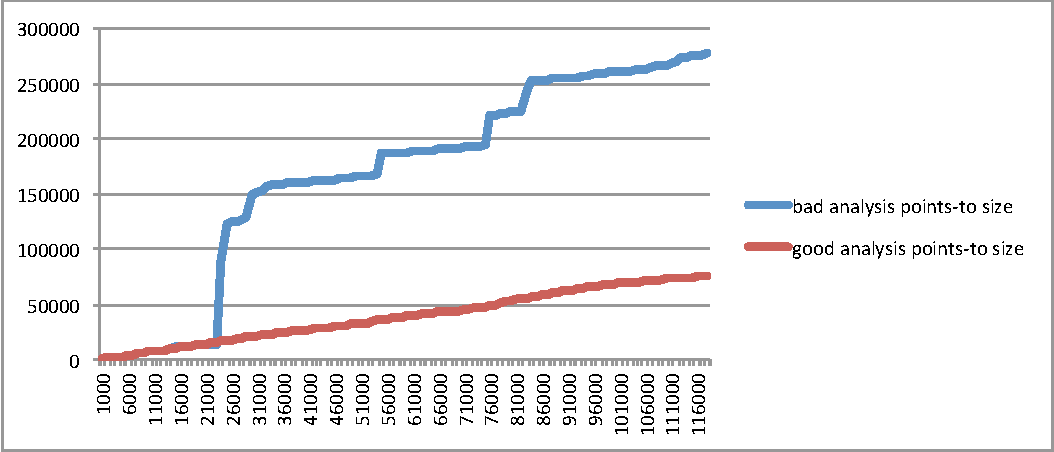
\includegraphics[width=\columnwidth]{pts-growth}
\caption{\textmd{Points-to size growth during the analysis lifetime.}}
\label{fig:pts-growth}
\end{figure}

Figure \ref{fig:pts-growth} shows the trend of overall points-to size (i.e., total number of points-to edges) growth for these two analyses during their lifetimes. The x axis presents the number of evaluations\footnote{An evaluation in the points-to analysis solves a constraint that may result in changes of the points-to results.} and y axis presents the total points-to size of all variables in the program. The good combined context-sensitive analysis' points-to size grows steadily ``linear'' throughout its lifetime. On the other hand, the overall points-to size growth of 0-1-CFA analysis exhibits ``jumps" which are the periods during which its overall points-to size dramatically increases. For example, between evaluations of 23,000 and 25,000, the overall points-to size of the 0-1-CFA analysis grows about ten times. The existence of such ``jumps" indicates that the overly-approximated results are frequently propagated, resulting in significantly overall precision loss. In addition, since the 0-1-CFA analysis experiences scalability issues, it remains incomplete at the end of the allocated analysis time and its overall points-to size keeps growing after the 120,000 evaluations in Figure \ref{fig:pts-growth}.

\begin{figure}[th!]
        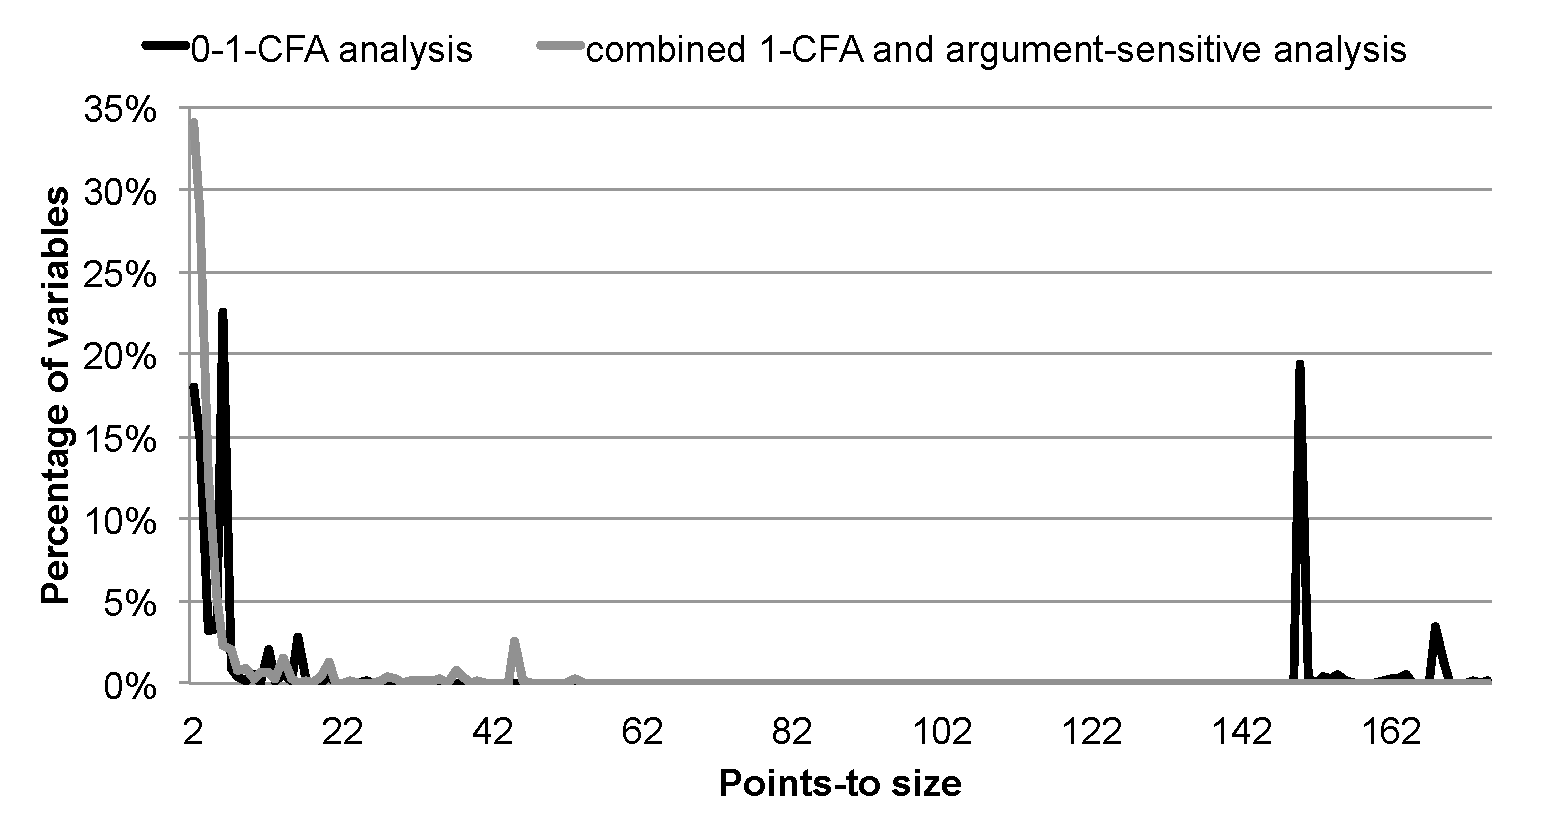
\includegraphics[width=\columnwidth]{pts-distribution}
\caption{\textmd{Points-to size distribution.}}
\label{fig:pts-distribution}
\end{figure}

Figure \ref{fig:pts-distribution} shows the distributions of the points-to sizes for each variable in the program. The x axis presents the points-to size of a variable and the y axis presents the percentage of the variables in the program with the corresponding points-to size. For the combined context-sensitive analysis, the points-to size of the majority of the variables (i.e., 81\%) is less than 6 and few variables are associated with large points-to sets. Interestingly for the 0-1-CFA analysis, the points-to sizes of only 40\% variables are less than 6 and there are condensed occurrences of variables with extremely large points-to sets (e.g., about 20\% of the variables' points-to sizes are 150). This result also indicates that overly-approximated results of specific program constructs may pollute many places in the program due to copying during the points-to propagations.

The above results demonstrate the significant different behaviors between points-to analyses when their performance and precision varies. These results motivated us to design an automated approach to identify root causes of imprecision via the differences of static analysis behavior. 

\subsection{Root Cause Localization \& Improvement Suggestion}

We now use the example in Figure \ref{fig:jquery-modified} to illustrate the ideas on localizing root causes. First, the root cause localization should be performed during the period in which overall precision of the points-to analysis starts to decrease, reflected as the ``jumps'' in terms of the overall points-to size in Figure \ref{fig:pts-growth}. Second, we use the history information of points-to propagations and the incomplete points-to results to locate the program constructs that are root causes of imprecision. Intuitively, two conditions should be met: (i) the program construct has a wide reach within the propagation system (e.g., the values of the property access {\tt source[name]} are assigned to property {\tt name} of {\tt target} at line 5 and are transitively propagated to about 500 other program variables or reference properties), and (ii) the impact of its wide reach is significant (e.g., looking up the property {\tt name} of {\tt source} at line 5 produces the points-to size of 150). Therefore, the imprecision of this property access results in the overall imprecision of the 0-1-CFA analysis when analyzing {\it jQuery} applications, becoming a root cause.

In addition, to further assist in the process of improving the results of static analysis, we design an improvement suggestion algorithm that uses dynamic information to suggest appropriate context sensitivity to improve the analysis precision on the identified root causes. The dynamic information is used to simulate the benefits of different context-sensitive analyses, a generally applicable idea to quantify the potential precision of a specific context sensitivity.

%because there are existing static analysis techniques that are designed to perform well for specific program constructs,

%Because of the high cost of locating analysis bottlenecks in programs, in this work we present automated bottleneck localization via program analysis based on the observations in terms of the points-to analysis behavior. We aim to locate the specific program variables as performance bottlenecks. Intuitively, two conditions should be met: 

%\begin{enumerate}
%	\item {\sf ptr} is (transitively) assigned to a large number of other pointer keys.
%	\item The points-to set of {\sf ptr} is large.
%\end{enumerate}
%By the first condition, {\sf ptr} has wide reach within the fixpoint system. By the second condition, the impact of its wide reach is significant. As an example, for 0-1-CFA analysis, looking up the property {\tt name} of {\tt source} at line 5 in Figure \ref{fig:jquery-modified} results in a large point-to set (i.e., 150 in size) and its values are assigned to property {\tt name} of {\tt target} and transitively to at least 30 other program variables. Therefore, the imprecision of this property accesses results in the overall imprecision of the 0-1-CFA analysis when analyzing {\it jQuery} applications, becoming an analysis bottleneck. Applying more accurate technique (e.g., \cite{Sridharan:2012:CTP:2367163.2367191}) at this specific program point may resolve the overall performance and precision issues. In this work, we have designed an automatic analysis that extracts the variable precision impact information from points-to analysis and locates the program locations that are analysis bottlenecks.

%In addition, we have also designed a automatic improvement suggestion algorithm that uses dynamic information to suggest appropriate context sensitivity to improve the analysis precision on bottlenecks. The dynamic information is used to animate the benefits of different context-sensitive analyses, a generally applicable idea to quantify the potential of context sensitivity precision on a subset of the functions in the program.

\begin{comment}
1. static analysis has issues with performance and precision, especially with dynamic features, and becomes useless.
    1.1 many JS analysis experiences performance issues; 
    1.2 it is difficult to manually reason about the causes of the issues (bottlenecks); 
    1.3 illustrate the second claim with example?
    
2. interesting behavior of useless analysis. 
     2.1 present the characteristics/behavior of useless and useful analysis, and compare.
     
3. the results from 2 lead us to design an analysis that analyzes the behavior of the useless analysis, (i) locates the bottlenecks, and (ii) propose possible fixes (with the same example)
\end{comment}

\begin{comment}
In this section, we walk the reader through an overview of our approach with reference to the code in Figure \ref{fig:jquery-extracted}, taken from the jQuery framework, for illustration purposes. [[ Can we say more about the example? ]]

\subsection{The Problem and Its Symptoms}

Static program analysis is challenged, by its very definition, by dynamic constructs like reflection. This is among the greatest challenges in JavaScript analysis, where reflective capabilities --- such as enumeration over, and access to, an object's properties --- are baked into the core syntax. Examples of this, in Figure \ref{fig:jquery-extracted}, are the {\sf for} loop iterating over property identifiers at lines XXX, YYY and ZZZ. Other challenging constructs include closures, variadic function, prototype-chain lookup, etc.

These (and other) challenges have significant impact on the precision of Andersen-style analysis of real-world JavaScript programs. In the absence of special treatment for challenging constructs, the analysis becomes overly conservative, losing track of correlations that are critical for acceptable precision. For the code in Figure \ref{fig:jquery-extracted}, for instance, the analysis would propagate pointers across every pair of properties in {\sf source} and {\sf target}, which is detrimental to its precision.

Importantly, however, at the lower level of the fixpoint system computing the points-to solution, these challenges are all abstracted into the same symptom: excessively large points-to sets due to infeasible pointer flows. As an illustration, 
we refer the reader to Figure \ref{fig:pts-growth}, which depicts the evolution of the points-to graph (measured as the number of points-to edges) for a simple client of jQuery v1.6.1 as a function of fixpoint iterations.

In the figure, there are two trend lines. The red ``linear'' line corresponds to 1-CFA analysis with argument sensitivity, and the other line to 0/1-CFA. As 0/1-CFA is more coarse, important dimensions of precision are lost, and the analysis fails to complete within a time budget of 10 minutes. Comparatively, the 1-CFA analysis finishes in under 5 seconds.

These behaviors are reflected in the trend lines. While the 1-CFA points-to graph grows at a steady rate, the 0-CFA line exhibits a jerky behavior with step-like jumps. These correspond to the symptoms mentioned above: large points-to sets reaching wide regions in the points-to graph.

\subsection{Step I: Diagnosis}

Our first observation, enabling diagnostic analysis, concerns the detemrmination whether a given pointer variable (or pointer key) {\sf ptr} is conducive to accuracy loss. For {\sf ptr} to qualify as such, two conditions should be met:
\begin{enumerate}
	\item {\sf ptr} is (transitively) assigned to a large number of other pointer keys.
	\item The points-to set of {\sf ptr} is large.
\end{enumerate}
By the first condition, {\sf ptr} has wide reach within the fixpoint system. By the second condition, the impact of its wide reach is significant.

As an example, ... [[ point to motivating example and show a fragment of points-to graph ]].

To enforce the diagnostic conditions above, we instrument the fixpoint system to track flow of pointer keys. Given a dataflow equation $e$ propagating points-to elements between pointer keys {\sf x} and {\sf y}, where {\sf y} has points-to set $S$, we instrument the points-to edge ${\sf y} \mapsto S$ to include {\sf x}: ${\sf y} \stackrel{{\sf x}}{\mapsto} S$.

Tracking pointer keys as edge labels addresses the first condition above. Evaluating the second condition is straightforward. Deriving the size of the points-to set of a given pointer key is immediate from the points-to graph.

\subsection{Step II: Remediation}

Having identified precision bottlenecks, in the form of pointer variables requiring additional sensitivity, we turn to the remediation problem. We propose a heuristic, based on (i) a parametric library of sensitivity policies as well as (ii) a dynamic analysis to simulate their effects w.r.t. concrete runtime states and compare between them, to recommend to the analysis designer how to refine the analysis.

\paragraph{Sensitivity Policies.} The problem of imprecision in JavaScript points-to graphs has been observed, and addressed, in various studies. Beyond that, there are general schemes to add sensitivity to a propagation-based call graph. In this paper, we focus on the following sensitivity policies in particular:
\begin{itemize}
	\item XXX
	\item YYY
	\item ZZZ
	\item ...
\end{itemize}

\paragraph{Recommendation Algorithm.} Given the library $\{ s_1,\ldots, s_n \}$ of sensitivity policies, the recommendation which (type of) sensitivity to add is based on simulating the effects of the different policies $s_i$ w.r.t. a fully concrete points-to graph computed dynamically. Policy $s$ is considered better than $s'$ if XXX.

The motivation for using dynamic analysis is to be able to quantify the precision loss, or ambiguity, introduced by a given policy. That is, we can reason fully precisely about the concrete points-to facts that are smushed together due to a given policy.

To compute the points-to graph dynamically, we instrument the JavaScript program. This is done via XXX. The instrumented program is, on average, xYYY slower compared to the original version. We handle XXX...

For the example in Figure \ref{fig:jquery-extracted}, our solution correctly picks ...




proceeds by instrumenting the subject program to record, at runtime, the concrete --- and thus fully precise --- points-to graph $G^c$. The question of which sensitivity to recommend to the analysis designer then 



\subsection{Motivating Example}
In this section, we would like to use a code example (or a series of examples; see below) to demonstrate the difficulties to (manually) find the performance bottleneck of a static analysis. For example, Figure \ref{fig:jquery-orig} shows the original {\tt extend} function of jQuery whose behavior is not easy to understand; moreover, due to its usage of complicated program structures (e.g., recursion, function variadicity), it is difficult for an analysis to accurately model the results of this function (confirmed in \cite{}). In \cite{}, the authors had to manually transform this function to simplify its structure, resulting in the code in Figure \ref{fig:jquery-modified}. Nevertheless, the transformed code, in and of itself, is still insufficient for a field-sensitive analysis to complete analyzing simple jQuery applications. Therefore, the authors of \cite{} designed an automatic function extraction algorithm (correlation extraction) and used argument sensitivity to improve the performance and precision of JavaScript points-to analysis. The code that is actually being analyzed by the argument-sensitive analysis is presented in Figure \ref{fig:jquery-extracted}. Overall, the take-away message shall be: it is difficult to locate the analysis bottleneck and it is also difficult to find a solution to improve the analysis. This series of examples strongly support the above statement: (1) among almost 9,000 lines of code of jQuery library, it usually is clueless to know that one particular function results in the analysis performance bottleneck (without investigating the code); (2) even if the analysis designer is able to locate this function as the bottleneck, it is difficult to tell which program structure or if it is the combination of several program structures that result in bad analysis behavior, thus making it difficult to develop new technology to improve the analysis; (3) even if the analysis designer is able to (manually) abstract away several challenges (e.g., the transformed function in Figure \ref{fig:jquery-modified}), and wants to apply the more precise technique whole program (e.g., argument sensitivity), this may in turn results in overhead because the other portion of the program may not benefit from the more advanced technique (although this particular function will significantly benefit from argument sensitivity). ({\bf Comment from Shiyi: despite that I think this is a good series examples as motivation, we cannot afford to use too much space for the codes; simplify the code, especially Figure 1 (included the complete code for your reference), as the ECOOP 12 paper did; or use one whole example to demonstrate what we want to express. Also, note that our technique does not automatically fixes the issues discussed in (1) and (2) above, while we do locate the bottleneck function and apply the advanced techniques, thus solving problem (3) above.}).

\begin{figure}[th!]
        \lstinputlisting{jquery-orig.js}
\caption{\textmd{Original {\tt extend} function of jQuery 1.6.1.}}
\label{fig:jquery-orig}
\end{figure}

\begin{figure}[th!]
        \lstinputlisting{jquery-extracted.js}
\caption{\textmd{Mofified {\tt extend} function with correlation extraction \cite{} of jQuery 1.6.1}}
\label{fig:jquery-extracted}
\end{figure}

\subsection{Static Points-to Analysis Behavior (Empirical Study)}
To (manually or automatically) understand and debug the performance and precision issues associated with static points-to analysis, it is important to know its behavior (normal and abnormal). We present some data to characterize the points-to analysis behavior.

1. growth of points-to graph size (points-to edges) during points-to analysis lifetime. Figure \ref{fig:pts-growth} shows the growth rate of two points-to analyses on an application that invokes jQuery 1.6.1 library. The bad points-to analysis is the baseline analysis (i.e., 0-1-cfa) which could not finish under limited time budget (10 minutes); the good points-to analysis is a 1-cfa and argument-sensitive which finishes analyzing the program in less than 5 seconds and the total number of points-to iteration is about 118,000. Comparing the life time of the bad (part of its lifetime as its lifetime could be much longer) and the good points-to analysis, we observe the growth rate of points-to size (i.e., we count the total number of points-to edges in the graph every 5000 iterations) of good points-to analysis is steady while the bad points-to analysis has ``jumps" (indicating the approximation and "pollution" of points-to results). This finding motivated us to design heuristics to decide when we would like to perform the automatic diagnostic analysis for a bad analysis (i.e., when the slope of growth significantly change). ({\bf Comment by Shiyi: the data of Figure \ref{fig:pts-growth} is included in section2-results.xlsx. I think this is interesting and we may need one more figure on other programs to better support our argument.})



2. Points-to size (per pointer key) distribution. See section2-results.xlsx for the data (columns I and J). The data show very interesting and different characteristics of points-to size distribution between a good and bad points-to analyses (the same analyses as in Figure \ref{fig:pts-growth}). We collected this data for each analysis after 100,000 iterations. I think we are looking for a frequency graph here that x axis represents the size of points-to size and y axis represents the number of pointer keys with the specific size of points-to set. Roughly looking at the data, for example in column I (the good points-to analysis), the curve is likely to evenly going down with the increase of points-to size. While for the bad points-to analysis (column J), the curve seems evenly going down with the increase of points-to size until the size of 33; after 33, the next size jumps to 150, and there are a lot of pointer keys with points-to size greater than 150 (thus, the frequency graph/curve/histogram would grow after specific number for the bad analysis). This result is interesting in that this indicates for a bad points-to analysis, some approximate results polluted a lot of places in the graph; thus making the analysis unscalable and extremely imprecise. ({\bf Comment by Shiyi: I can use excel to generate the frequency graph, but it may take some time for me to do so, but I do think this result is interesting to report because the "outliers" (i.e., many pointer keys with large points-to size) in the bad points-to graph indicate how the bottleneck can pollute the analysis and that motivates us find the bottleneck. Furthermore, taking close look at the "large" points-to sizes, many pointer keys share the same points-to sizes, indicating that many could be copies from previously approximate results; thus being "polluted" after copying. This finding motivates us to track the copies of points-to sets during the diagnosis.})

3... We may think of more to report on points-to analysis characteristics. We shall focus on the characteristics that distinguish the good and bad points-to analysis. More data make this subsection an empirical study of static points-to analysis behavior and characterization of good/bad points-to analysis, which in and of itself is a good effort and something new to present, thus making it a contribution of this paper.

({\bf Further comments on Section 2 by Shiyi: I think with the empirical study, this section can be long, but it is Ok as we already are presenting new observations and findings in this section. These new findings very well serve the motivation and design guidance of our algorithm; thus very tightly connected to the rest of the paper.})
\end{comment}

\section{Overview \& Design}
\label{design}

\begin{figure}[th!]
        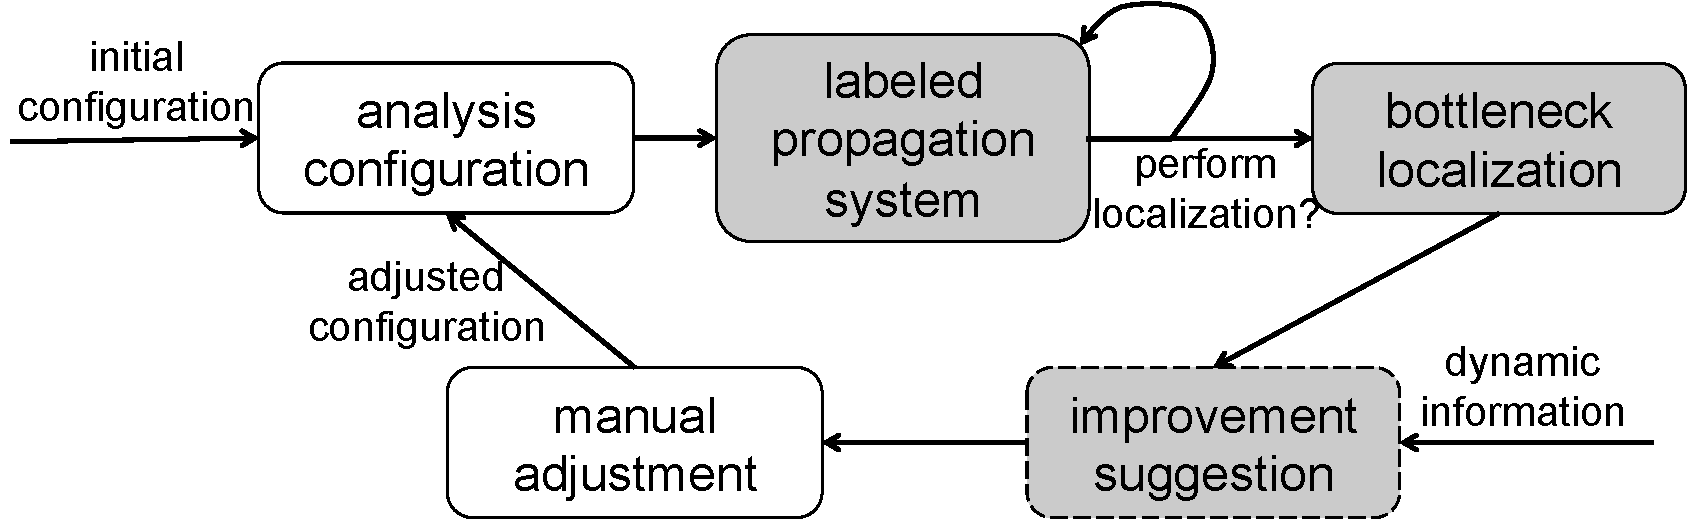
\includegraphics[width=0.9\columnwidth]{overview}
\caption{\textmd{Root cause localization process overview.}}
\label{fig:overview}
\end{figure}

{\bf Algorithms.}

\begin{algorithm}[th!]
\begin{algorithmic}[1]
{
\renewcommand{\algorithmicrequire}{\textbf{Input:}}
\renewcommand{\algorithmicensure}{\textbf{Output:}}
\REQUIRE {\tt config}: analysis configuration
\REQUIRE {\tt i}: evaluation interval
\ENSURE {\tt R}: set of root causes
\STATE {\tt sys} $\leftarrow$ initialize propagation system with {\tt Config}
\WHILE{({\tt c} $\leftarrow$ next constraint in {\tt sys}) != NULL //fixed-point has not been reached} 
%\STATE {\tt pts} $\leftarrow$ points-to propagation on {\tt c}
\FOR{each points-to assignment {\tt v1 = v2} from {\tt c}}
\STATE {\tt pts\textsubscript{v1}= pts\textsubscript{v1} $\bigcup$ pts\textsubscript{v2}} //points-to propagation
\STATE {\tt l\textsubscript{v1} = l\textsubscript{v1} $\bigcup$ l\textsubscript{v2} $\bigcup$ \{v2\}} //label propagation
\ENDFOR
\IF{{\tt (k $\leftarrow$ No. of evaluations) mod i = 0}}
\STATE  grow $\leftarrow$ points-to size growth in past {\tt i} evaluations
\IF{grow > threshold //to perform localization when the growth rate is high}
\STATE g $\leftarrow$ intermediate points-to graph with labels //do not require a complete graph
\FOR{each pointer key node {\tt n} in {\tt g}}
\STATE impact\textsubscript{n} $\leftarrow$ compute the impact of {\tt n} on {\tt g}
\ENDFOR
\STATE V $\leftarrow$ nodes with high impacts
\RETURN
\ENDIF
\ENDIF
\ENDWHILE
}
\end{algorithmic}
\caption{Root cause localization workflow.}
\label{alg:localization}
\end{algorithm}

\begin{algorithm}[th!]
\begin{algorithmic}[1]
{
\renewcommand{\algorithmicrequire}{\textbf{Input:}}
\renewcommand{\algorithmicensure}{\textbf{Output:}}
\REQUIRE {\tt R = \{r\textsubscript{1}, ..., r\textsubscript{n}\}}: root causes
\REQUIRE: {\tt t}: dynamic trace
\ENSURE {\tt <V, S>=\{(r\textsubscript{1}, s\textsubscript{1}),...,(r\textsubscript{n}, s\textsubscript{n})\}}: suggestions
\STATE G $\leftarrow$ taking {\tt t} as input, create a set of dynamic points-to graphs with different context sensitivity policies //some operations from Procedure 3 may be moved here
\FOR{each {\tt r\textsubscript{i}} $\in$ {\tt R}}
\STATE A\textsubscript{<r\textsubscript{i}, G>} $\leftarrow$ $\emptyset$ 
\FOR{each {\tt g\textsubscript{j}} $\in$ {\tt G}}
%\STATE |pts\textsubscript{(r, g)}| $\leftarrow$ query {\tt r}'s total points-to size in {\tt g}
%\STATE |cs\textsubscript{(r, g)}| $\leftarrow$ query number of calling contexts for {\tt r} in {\tt g}
\STATE a\textsubscript{<r\textsubscript{i}, g\textsubscript{j}>} $\leftarrow$ query {\tt r\textsubscript{i}}'s total points-to size in {\tt g\textsubscript{j}} and measure its accuracy corresponding to {\tt g\textsubscript{j}}'s context sensitivity policy
\STATE A\textsubscript{<r\textsubscript{i}, G>} = A\textsubscript{<r\textsubscript{i}, G>} $\bigcup$ \{a\textsubscript{<r\textsubscript{i}, g\textsubscript{j}>}\}
\ENDFOR
\STATE a\textsubscript{<r\textsubscript{i}, g>} $\leftarrow$ min(A\textsubscript{<r\textsubscript{i}, G>}) //pick the dynamic points-to graph on which r\textsubscript{i} is the most accurate
\STATE <V, S> = <V, S> $\bigcup$ \{<r\textsubscript{i}, g's context sensitivity>\}
\ENDFOR
}
\end{algorithmic}
\caption{Improvement suggestion workflow.}
\label{alg:suggestion}
\end{algorithm}

\subsection{Overview}

{\bf TODO: re-order the boxes in Figure \ref{fig:overview}.}

Figure \ref{fig:overview} shows an overview of the root cause localization process with the support of our automatic approaches. We first initialize the static analysis with an initial configuration in terms of context sensitivity, which experiences poor performance and/or precision behavior. The initial analysis is performed on the target program under a {\it labeled propagation system} which keeps track of the history of point-to propagations, labeling the origins of the points-to relations. Moreover, instead of waiting until the analysis achieves a fixed-point,\footnote{An analysis that experiences scalability issues on a program often cannot achieve the fixed-point within the time budget. This design allows us performing root cause localization on intermediate states during the points-to propagations.} we periodically pause the propagation system to evaluate the intermediate states. Heuristics are used to decide whether to perform {\it root cause localization} (i.e., when the abnormal behavior is observed); if not, the points-to propagations are resumed. The root cause localization identifies a set of variables and/or reference properties in the program as root causes of imprecision, using the points-to analysis history information collected by the labeled propagation system. The algorithm ranks the results in order of their impact to the overall analysis precision and therefore indicating their possibilities of being the root causes.

The optional {\it improvement suggestion} stage takes the localized root causes as inputs to automatically generate suggestions to improve the analysis with specialized context-sensitive analysis. The suggestions are based on the dynamic information. We collect in advance a dynamic trace of the program execution and compute dynamic points-to graphs based on the run-time information with pre-defined context sensitivity. Finally, a user (i.e., program analysis designer) may manually adjust the analysis configuration based on the localization results and/or the improvement suggestions. Furthermore, the analysis can be re-run under the adjusted configuration to observe if the performance and/or precision issues have been resolved. The same process may be performed multiple times to locate all the root causes and develop a specialized analysis configuration that would result in desired analysis performance and precision.

\subsection{Labeled Propagation System}

A propagation system for the points-to analysis solves the constraints to reach the fixed-point, propagating the points-to relations of the variables and reference properties in the program. A majority of the constraints that exist in the propagation system are assignments. For example, to process an invoke instruction, the generated constraints include assignments from the actual arguments to the formal parameters, from the callee's return values to the left-hand side variable of the invoke instruction, etc. The propagation system solves a constraint that assigns a variable {\tt v1} to another variable {\tt v2} by adding the points-to set of {\tt v1} to that of {\tt v2}. The results of such constraint propagations are therefore reflected in the points-to results. However, when the points-to set of a variable or a reference property is queried, the history information of the points-to relations is lost, which may originate from multiple transitive assignments. Such information is critical for identifying root causes because frequent assignments from an inaccurate points-to set may pollute the overall precision of the points-to analysis as indicated by the results in Figures \ref{fig:pts-growth} and \ref{fig:pts-distribution}.

In our labeled propagation system, each constraint that assigns the values of {\tt v1} to {\tt v2} results in not only the changes to {\tt v1}'s points-to relations but also a label {\tt v2} associated with the points-to set of {\tt v1} indicating the points-to relations of {\tt v1} were propagated from {\tt v2}. For example, the WALA's SSA IR represents the statement at line 5 in Figure \ref{fig:jquery-modified} as (a) {\tt v\textsubscript{tmp} = source[name]} and (b) {\tt target[name] = v\textsubscript{tmp}}, where {\tt v\textsubscript{tmp}}, {\tt source}, {\tt target} and {\tt name} are all local variables of the function.  For the property read instruction (a), the analysis would first query the points-to set of {\tt source}, {\tt P\textsubscript{source}}, and the points-to set of {\tt name}, {\tt P\textsubscript{name}}. The pairs of each element in {\tt P\textsubscript{source}} and {\tt P\textsubscript{name}} (e.g., {\tt p\textsubscript{source\_i}.p\textsubscript{name\_j}}) are returned as the results of looking up the reference properties of {\tt source[name]}. Note that the values of {\tt name} iterate over all the property names of {\tt source}, which in practice are the large set of the function names loaded in {\it jQuery}. It eventually results in a large points-to set for {\tt v\textsubscript{tmp}} due to multiple assignments from various reference properties and we keep all these reference properties (e.g., {\tt p\textsubscript{source\_i}.p\textsubscript{name\_j}}) as labels for the points-to set of {\tt v\textsubscript{tmp}}. For the property write instruction (b), the analysis similarly looks up the reference properties of {\tt target[name]} (e.g., {\tt p\textsubscript{target\_i}.p\textsubscript{name\_j}}) and adds the points-to relations of {\tt v\textsubscript{tmp}} to each of these reference properties, resulting in overly-approximated points-to set for each function name of {\it jQuery}. We keep both {\tt v\textsubscript{tmp}} and the transitively existing labels from {\tt v\textsubscript{tmp}} (e.g., {\tt p\textsubscript{source\_i}.p\textsubscript{name\_j}}) for the points-to set of each reference property of {\tt target[name]}.

More interestingly, in addition to tracking the set of labels that are immediately or transitively propagated to the points-to set of a variable or a reference property, we generate a {\it propagation-history graph} for the points-to set of each variable and reference property, which represents the hierarchical information of the points-to propagation history. Intuitively, a node in the propagation-history graph is a variable or a reference property that has an impact on the specific points-to set. An edge from a node {\tt n\textsubscript{1}} to another node {\tt n\textsubscript{2}} represents that the points-to set of {\tt n\textsubscript{2}} was explicitly added to that of {\tt n\textsubscript{1}}. The entry points of the graph are the variables and/or reference properties whose points-to sets are directly propagated into the corresponding points-to set. For the same example in Figure \ref{fig:jquery-modified}, the propagation-history graph for the points-to set of {\tt v\textsubscript{tmp}} consists of all the reference properties of {\tt source[name]} as entry points. {\tt v\textsubscript{tmp}} is the entry point of the propagation-history graph for the points-to set of each reference property of {\tt target[name]} (e.g., {\tt p\textsubscript{target\_i}.p\textsubscript{name\_j}}), while there also are edges from {\tt v\textsubscript{tmp}} to the properties of {\tt source[name]}.

\subsection{Root Cause Localization}

\begin{figure}[th!]
        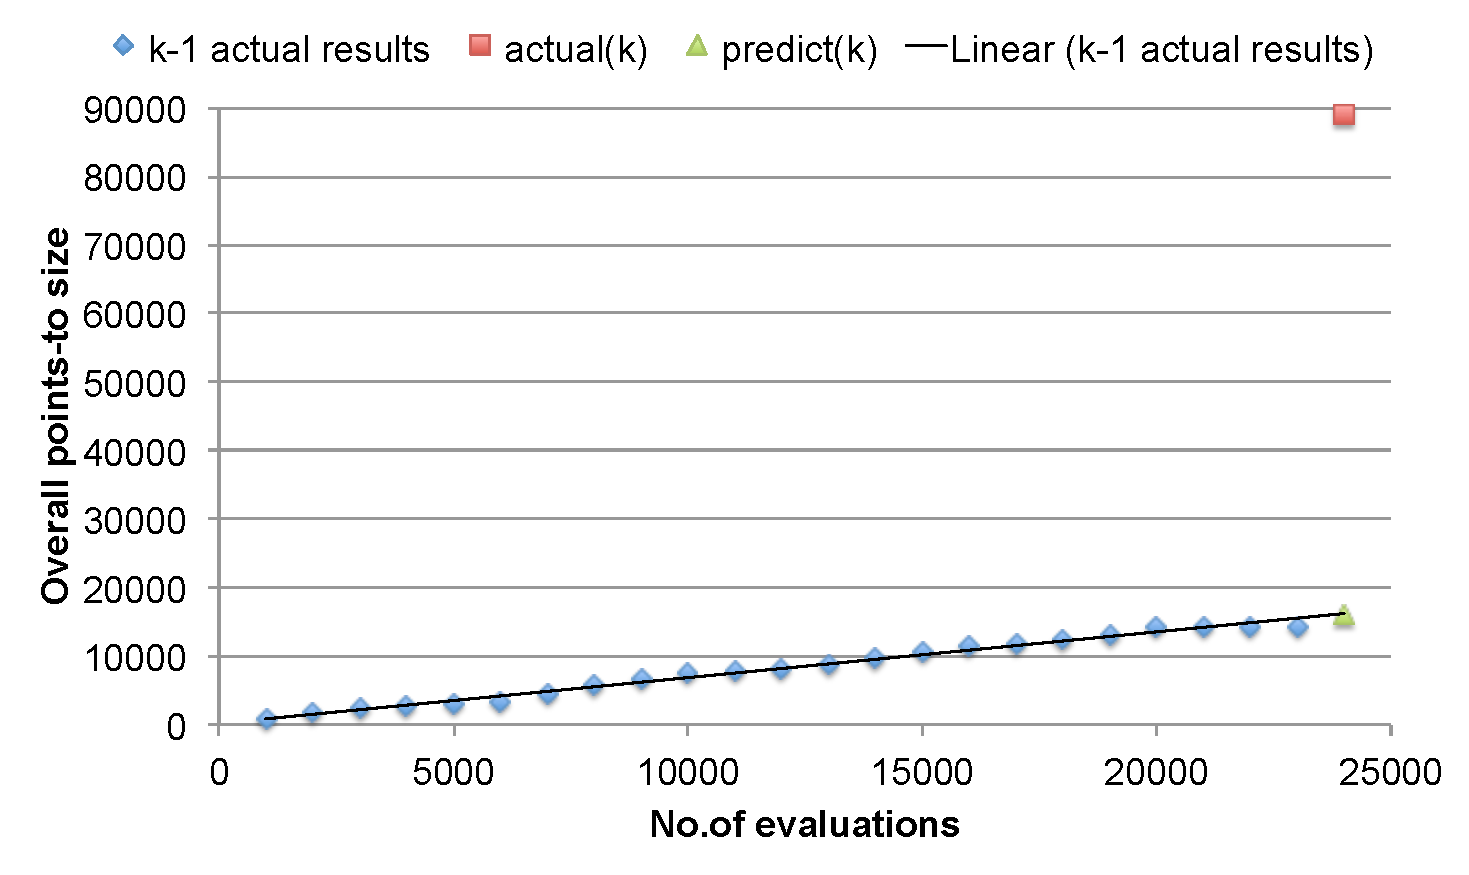
\includegraphics[width=\columnwidth]{linear}
\caption{\textmd{Prediction via linear regression.}}
\label{fig:linear}
\end{figure}

During the process, the labeled propagation system is paused every {\tt n} evaluations. We use the intermediate states to decide whether root cause localization is performed. We count the total number of points-to relations (i.e., edges) in the intermediate points-to graph for the {\tt k\textsubscript{th}} pause (i.e., after {\tt n$\times$k} evaluations), {\tt actual(k)}. We compare the value of {\tt actual(k)} with the value of {\tt predict(k)} to decide on whether to perform root cause localization. Using intermediate results from the previous {\tt k-1} pauses, we perform a simple linear regression to find the fitted line {\tt y = intercept + slope $\times$ x}, where {\tt x} is the number of evaluations and {\tt y} is the total number of points-to relations. Therefore, the number of points-to relations of the {\tt k\textsubscript{th}} pause can be predicted: {\tt predict(k) = intercept + slope $\times$ kn}. If {\tt actual(k) > 110\% $\times$ predict(k)}, we decide to perform the root cause localization at the {\tt k\textsubscript{th}} pause; otherwise, we continue the points-to analysis under the labeled propagation system. Figure \ref{fig:linear} shows this prediction model running the 0-1-CFA analysis on a {\it jQuery} application. The analysis is paused every 1000 evaluations and the fitted line in Figure \ref{fig:linear} is calculated from the results of the first 23 pauses (i.e., 1000 to 23,000 evaluations). The predicted total points-to edges at the 24,000 evaluations is 16,234, while {\tt actual(24)} is 88,857, significantly passing the threshold to perform the root cause localization. This prediction model can capture the ``jump'' period of the points-to analysis shown in Figure \ref{fig:pts-growth} and is important for accurately localizing the root causes. If the localization is performed too early, the overly-approximated results may have not surfaced. If the localization is performed late during the analysis, the overly-approximated results of the root causes may have polluted a large portion of the overall points-to results, making it difficult to identify the root causes of imprecision. Moreover, the evaluation interval to pause the analysis, {\tt n}, as well as the decision threshold may be tuned based on the budget and goals of root cause localization.

%During the progress, the label propagation system is paused periodically. The intermediate results are used to decide whether bottleneck localization is performed, using the predicted value of linear regression. A linear regression is predicted based on the {\tt k-1} pauses. If the actual value of the {\tt k}'s pause is greater than 110\% of the predicted value, we determine that the analysis may have entered the ``jump" period shown in Figure \ref{fig:pts-growth} and the bottleneck localization is performed.

When performing root cause localization, we use the intermediate points-to graph and the associated labels to identify possible root causes. For each variable or reference property {\tt v}, we count (i) its points-to size, {\tt |P\textsubscript{v}|}, and (ii) its number of occurrences as labels in the points-to sets of other variables and/or reference properties, {\tt |L\textsubscript{v}|}. {\tt |L\textsubscript{v}|} measures how widely {\tt v} reaches within the propagation system and {\tt |P\textsubscript{v}|} measures if the impact of its wide reach is significant. We therefore use the score {\tt S\textsubscript{v}=|P\textsubscript{v}|$\times$|L\textsubscript{v}|} as a measurement of the possibility of {\tt v} being the root cause. The root cause localization stage reports a set of variables as root causes in descending order of their scores. For example, {\tt v\textsubscript{tmp}}, the result of the property read instruction at line 5 in Figure \ref{fig:jquery-modified}, has a extremely high score (73,950) with {\tt |P\textsubscript{v\textsubscript{tmp}}|=150} and {\tt |L\textsubscript{v\textsubscript{tmp}}|=493} when the root cause localization is performed after the 24,000 evaluations. Its score is 75 times higher than the variable with the second highest score (990), making it the only candidate as the root cause of imprecision of 0-1-CFA analysis for this {\it jQuery} application. We report the variables and/or reference properties whose scores are at least 50\% the highest score as {\it suspicious root causes}.

%We then assign score to each variable and/or reference property by calculating (i) $\times$ (2). The higher score indicates the variable is more likely to be analysis bottlenecks. We report the variables with scores great than half of the one with the highest scores.

\subsection{Improvement Suggestion}

We have discussed the approaches that automatically identifies the root causes of imprecision. A user may manually adjust the analysis to improve the analysis precision on these root causes. More automatic support on suggesting possible analysis configurations will further assist in improving the analysis precision on the program. We present automatic improvement suggestion in terms of a specialized context-sensitive analysis.

First, the target program is executed to collect a dynamic trace, recording the following run-time information in order of occurrence: (i) function enters and exits, (ii) invocations, and (iii) property reads and writes. At a property read or write instruction we record (i) the instruction location in the program, (ii) the allocation site (in terms of the program location) of the base object, (iii) the property name, and (iv) the allocation site of the value if it is a reference object or the type of the value if it is primitive. At an invoke instruction we record (i) the location of the call site, (ii) the location of the target function, (iii) the allocation site of the receiver object, and (iv) the allocation sites and/or the types of the actual arguments. Second, dynamic points-to graphs based on the dynamic trace are generated under various kinds of context sensitivity. Procedure \ref{alg:dyn-pts} shows the algorithm that produces a dynamic points-to graph with respect to a specific context-sensitive analysis (e.g., 1-CFA, argument-sensitive or context-insensitive analysis). It takes the dynamic trace, {\tt Trace}, and the kind of context sensitivity, {\tt CS}, as inputs. The algorithm iterates through all the instructions recorded in the dynamic trace. For each instruction {\tt i}, the algorithm examines its kind. If it is an invoke instruction, at line 5, the call site and the argument are pushed into the call stack, {\tt Stack}. If it exits a function, the top element of {\tt Stack} is removed  at line 7. If it is a property read or write instruction, at lines 9 to 15, depending on the input context sensitivity, the calling context, {\tt Context}, is determined by the call site and the argument from the top element of {\tt Stack} for 1-CFA and argument-sensitive analysis, respectively; the calling context is {\it everywhere} for context-insensitive analysis. In the dynamic points-to graph, a variable is represented by (i) the location of the instruction, (ii) the part of the instruction (i.e., base, property or value), and (iii) the calling context. At lines 16 to 18, the object allocation site, represented by program location, of each part of the instruction collected at runtime is assigned to the corresponding variable node in the dynamic points-to graph. Note that this algorithm is general in that various dynamic points-to graphs that can be generated under different context sensitivity.
%The ultimate goal of our proposed approach is to improve the performance and/or precision of the analysis on the program. The identified bottlenecks are the program constructs 

\newcommand{\SWITCH}[1]{\STATE \textbf{switch} (#1) \begin{ALC@g}}
\newcommand{\ENDSWITCH}{\end{ALC@g} \STATE \textbf{end switch}}
\newcommand{\CASE}[1]{\STATE \textbf{case} #1\textbf{:} \begin{ALC@g}}
\newcommand{\ENDCASE}{\end{ALC@g}}
\newcommand{\CASELINE}[1]{\STATE \textbf{case} #1\textbf{:} \begin{ALC@g}}
\newcommand{\DEFAULT}{\STATE \textbf{default:} \begin{ALC@g}}
\newcommand{\ENDDEFAULT}{\end{ALC@g}}
\newcommand{\DEFAULTLINE}[1]{\STATE \textbf{default:} }

\begin{algorithm}[th!]
\floatname{algorithm}{Procedure}
\begin{algorithmic}[1]
{
\renewcommand{\algorithmicrequire}{\textbf{Input:}}
\renewcommand{\algorithmicensure}{\textbf{Output:}}
\REQUIRE {\tt Trace}: dynamic trace; {\tt CS}: context sensitivity
\ENSURE {\tt G}: dynamic points-to graph
\STATE {\tt Stack = empty}
\WHILE{{\tt (i = next(Trace)) != NULL}}
\SWITCH {{\tt kindOf i}}
\CASE {{\tt INVOKE}}
 \STATE  {\tt Stack.push(Pair(i\textsubscript{callsite}, i\textsubscript{arg1}))}
 \ENDCASE
\CASELINE {{\tt FEXIT}}
 \STATE  {\tt Stack.pop}
 \ENDCASE
  \CASELINE {{\tt PREAD || PWRITE}}
  \IF{{\tt CS = 1-CFA}}
\STATE {\tt Context = S.top().fst}
\ELSIF{{\tt CS = argument-sens}}
 \STATE {\tt Context = S.top().snd}
 \ELSIF{{\tt CS = context-insens}}
 \STATE {\tt Context = everywhere}
\ENDIF
\STATE {\tt G\textsubscript{(i\textsubscript{loc},base,Context)} $\rightarrow$ i\textsubscript{base}}
\STATE {\tt G\textsubscript{(i\textsubscript{loc},property,Context)} $\rightarrow$ i\textsubscript{property}}
\STATE {\tt G\textsubscript{(i\textsubscript{loc},value,Context)} $\rightarrow$ i\textsubscript{value}}
 \ENDCASE
\ENDSWITCH
\ENDWHILE
}
\end{algorithmic}
\caption{Dynamic points-to graph generation.}
\label{alg:dyn-pts}
\end{algorithm}

Now that we have obtained the dynamic points-to graphs under different context-sensitive analyses (i.e., 1-CFA, argument-sensitive and context-insensitive). For a variable {\tt v} that is identified as a root cause, we locate its corresponding nodes via its program location in each dynamic points-to graph and collect (i) the number of calling contexts associated with {\tt v}, {\tt |CS|}, and (ii) the sum of points-to sizes under all calling contexts, {\tt $\sum$|P\textsubscript{v}|}. We then count {\tt D\textsubscript{v} = $\sum|P\textsubscript{v}|\over |CS|$}, the average dynamic points-to size per calling context, to measure the accuracy of the points-to relations of {\tt v} under the specific context sensitivity. The context sensitivity under which {\tt D\textsubscript{v}} is the smallest is chosen for the function that contains {\tt v} as the improvement suggestion.

{\bf TODO: discussions on why using dynamic information and the impact of its incompleteness.} 

\section{Evaluation}
\label{evaluation}

We have conducted experiments to demonstrate the effectiveness of our approach. In this section, we present the experimental results of our analysis on various JavaScript benchmarks.

%We conducted three sets of experiments to demonstrate several aspects of our analysis. (1) the ability for the localization algorithm to pinpoint the critical bottleneck of the analysis on JavaScript libraries, (2) further experiments of the localization algorithm on JavaScript benchmarks and demonstrate the ability of suggestion algorithm, and (3) a case study on using our analysis to localize the issues of an unscalable and imprecise analysis for analyzing jQuery, and demonstrate that with manual modifications of the program without changing the semantics, the same analysis manages to be scalable on analyzing the jQuery programs.
\begin{comment}
\begin{table*}[h!]
\centering
\begin{tabular}{ | C{0.68in} | C{0.4in} | C{0.4in} | C{0.4in} | C{0.4in} | C{0.4in} | C{0.4in} | C{0.4in} | C{0.4in} | C{0.4in} | C{0.4in} | C{0.4in} |}
\hline
 {\bf library} & \multicolumn{3}{|c|}{\bf baseline} &  \multicolumn{4}{|c|}{\bf straw man} &  \multicolumn{4}{|c|}{\bf selective}\\
 \hline
 & {\tt REAC\_} {\tt FUNC} & {\tt AVG\_} {\tt TARG} & {\tt HIGH\_} {\tt POLY} & {\tt REAC\_} {\tt FUNC} & {\tt AVG\_} {\tt TARG} & {\tt HIGH\_} {\tt POLY} & time (sec) & {\tt REAC\_} {\tt FUNC} & {\tt AVG\_} {\tt TARG} & {\tt HIGH\_} {\tt POLY} & time (sec)\\ 
 \hline
jQuery & 291 & 20.1 & 272 & 206 & 1.2 & 21 & 17.3 & 206 & 1.2 & 16 & 16.9\\
 \hline
 prototype.js & 418 & 12.3 & 124 & 170 & 1.3 & 18 & ~2.9 & 170 & 1.3 & 18 & ~3.2\\
 \hline
 yui & 244 & ~9.8 & 124 & 101 & 1.1 & ~2 & ~1.1 & 101 & 1.1 & ~2 & ~2.0 \\
 \hline
 \end{tabular}
\caption{\textmd{Benchmarks I precision and performance results.}}
\vspace{-6pt}
\label{table:b1-precision-time}
\end{table*}
\end{comment}

\begin{table*}[th!]
\centering
\begin{tabular}{ | C{0.80in} | C{0.4in} | C{0.4in} | C{0.4in} | C{0.4in} | C{0.4in} | C{0.4in} | C{0.4in} | C{0.4in} | C{0.4in} | C{0.4in} |}
\hline
 {\bf library} & \multicolumn{3}{|c|}{\bf 1-CFA} &  \multicolumn{3}{|c|}{\bf 1-CFA + 1st-arg-sens} &  \multicolumn{4}{|c|}{\bf 1-CFA + selective 1st-arg-sens}\\
 \hline
 & {\tt REAC\_} {\tt FUNC} & {\tt AVG\_} {\tt TARG} & {\tt HIGH\_} {\tt POLY} & {\tt REAC\_} {\tt FUNC} & {\tt AVG\_} {\tt TARG} & {\tt HIGH\_} {\tt POLY} &  {\tt REAC\_} {\tt FUNC} & {\tt AVG\_} {\tt TARG} & {\tt HIGH\_} {\tt POLY} & time (sec)\\ 
 \hline
jQuery & 312 & ~2.2 & 441 & 206 & 25.0 & 1235 & 206 & 1.2 & 16 & 16.3\\
 \hline
 prototype.js & 451 & 12.9 & 259 & 170 & ~3.3 & ~124 & 170 & 1.5 & 39 & ~2.9\\
 \hline
 script.aculo.us & 617 & 14.4 & 188 & 179 & ~2.7 & ~145 & 179 & 1.4 & 47 & ~4.6 \\
 \hline
 \end{tabular}
\caption{\textmd{Benchmarks I precision and performance results.}}
\vspace{-6pt}
\label{table:b1-precision-time}
\end{table*}

\subsection{Experimental Setup} 

\subsubsection{Metrics}

In our evaluation, we compare the performance and precision of points-to analysis. A JavaScript points-to analysis usually constructs a call graph as well as a points-to graph. For precision on a call graph, we measure (i) {\tt HIGH\_POLY}: the number of highly polymorphic call sites (i.e., call sites with more than 5 targets), (ii) {\tt AVG\_TARG}: the number of targets averaged over all call sites, and (iii) {\tt REAC\_FUNC}: the number of reachable functions. The {\tt HIGH\_POLY} and {\tt REAC\_FUNC} metrics were also used by Sridharan et al. \cite{Sridharan:2012:CTP:2367163.2367191} to evaluate the call graph construction algorithms. For precision on a points-to graph, we measure {\tt PTS\_SIZE}: the overall points-to size (i.e., the total number of points-to set sizes over all local variables in the program; the points-to set of a variable is the number of abstract objects, represented by the allocation sites, it refers to). 
%For each of the above metrics, if an analysis $A_1$ produces smaller results than another analysis $A_2$, $A_1$ is more precise than $A_2$ on that aspect of the call graph or points-to graph.
In addition, we measure the performance of the points-to analysis with its running time (in seconds).

%{\bf Call graph metrics.} no. of high polymorphic call sites, average no. of targets, reachable functions

%{\bf Points-to graph metrics.} overall points-to size

\subsubsection{Benchmarks}

We use two sets of JavaScript benchmarks in our evaluation.
%For the JavaScript benchmarks experiments presented in Section \ref{}, we used the benchmarks collected by Kashyape \cite{}. There are 28 programs in the benchmarks that are divided into 4 categories. As demonstrated by Wei and Ryder \cite{}, programs from different categories can benefit from different context-sensitive analysis; thus in our experiments, we compared the precision and performance of whole-program context-sensitive analyses with the selective context-sensitive analysis to demonstrate the effectiveness of our bottleneck localization.

%For the JavaScript library experiments presented in Section \ref{}, we used the benchmarks developed by Srihadran \cite{}. The libraries that we evaluated are jQuery, prototype.js, and .... Because there is no existing analysis in WALA can scale (given the budget of 10 minutes) to analyze the simple applications that use the original versions of these libraries, we use manually transformed versions of these libraries which scale only with the analysis presented by Srihadran \cite{}. Each of the libraries is associated with several simple applications.

%For the previous two experiments, we have used a specific version of WALA to perform the evaluation. In the current WALA, there exist no analysis that can finish analyzing the programs used in the second experiments. In our case study presented in Section \ref{}, we use our bottleneck localization algorithm to pinpoint the places the these library applications that the current WALA analysis resulted in significant imprecision and manually transform the programs without changing their semantics so that the analysis is more precise on analyzing the transformed programs. A similar approach is used by Srihadran \cite{} to investigate the effectiveness of correlation tracking analysis.

{\bf Benchmarks I.} Benchmarks I consists of applications that use JavaScript libraries, generated by Sridharan et al. \cite{Sridharan:2012:CTP:2367163.2367191}. In this benchmark, there are 11, 5 and 1 simple web applications that invoke {\it jQuery}, {\it prototype.js} and {\it script.aculo.us} libraries, respectively. These libraries are among the most popular JavaScript libraries for developing real-world web applications, especially {\it jQuery} \cite{LibraryUsage}. As reported by Sridharan et al. \cite{Sridharan:2012:CTP:2367163.2367191}, an analysis without the specialized argument sensitivity experienced severe performance and precision problems; it required advanced static analysis techniques as well as manual code rewriting for improving precision and performance. In our experiments, we reuse these libraries with these manual transformations.

{\bf Benchmarks II.} Benchmarks II are JavaScript applications collected by Kashyap et al. \cite{Kashyap:2014:JSA:2635868.2635904}. Twelve out of the 28 programs from the original benchmarks were selected for our evaluation. These programs are collected from open-source JavaScript repositories, standard JavaScript benchmarks (e.g., SunSpider\footnote{https://webkit.org/perf/sunspider/sunspider.html}), and the Emscripten LLVM test suite\footnote{http://kripken.github.io/emscripten-site/}, the results of which benefit from various context-sensitive analyses \cite{Kashyap:2014:JSA:2635868.2635904,DBLP:conf/ecoop/WeiR15}.

\subsubsection{Experimental Design} 
%We have designed experiments to illustrate the effectiveness of the important aspects of our approach.

{\bf Root-cause localization.} We perform experiments on Benchmarks I to illustrate the accuracy of the root-cause localization algorithm. In this experiment, we use WALA's whole-program 1-CFA analysis as the {\it baseline} analysis, which experiences scalability and precision problems for the JavaScript library applications. For each of the Benchmark I programs, we perform the localization algorithm on the 1-CFA analysis, localizing a set of functions that contain the root causes. We then apply additional argument sensitivity on the first arguments (i.e., 1st-argument sensitivity \cite{DBLP:conf/ecoop/WeiR15}) of all these functions; for the rest of the functions, the 1-CFA analysis is performed (i.e., a 1-CFA and {\it selective} 1st-argument-sensitive analysis). We compare the precision results among the 1-CFA, the whole-program 1-CFA and 1st-argument-sensitive analysis, and the {\it selective} analysis using the call graph metrics for Benchmarks I. We also compare the differences in terms of analysis performance.

%In our experiments, we use WALA's whole-program 1-CFA and 0-1-CFA JavaScript points-to analyses\footnote{For the results reported in Sections \ref{b1-res} and \ref{b2-res}, we conducted the experiments based on analyses implemented under WALA version R\_1.3.4. We performed the case studies in Section \ref{case-study} using the up-to-date WALA implementations to locate and understand the root causes.} as the {\it baseline} analyses for Benchmarks I and Benchmarks II, respectively. The 1-CFA analysis experiences scalability and precision problems for the JavaScript library applications in Benchmarks I and the 0-1-CFA analysis is imprecise for the programs in Benchmarks II comparing to other analyses in comparison. A whole-program combined context-sensitive analysis (i.e., 1-CFA and argument sensitivity) applies the more accurate but also more expensive context sensitivity policy. 

%{\bf Root-cause localization.} To illustrate the accuracy of the root-cause localization approach, for each of the benchmark programs, we perform the localization algorithm on the {\it baseline} analysis where performance and/or precision problems are present. We apply 1-CFA analysis and combined 1-CFA and argument-sensitive analysis on all the functions that contain the identified root causes for Benchmarks I and Benchmarks II, respectively; for the rest of the functions, the {\it baseline} analysis is performed (i.e., a {\it selective} context-sensitive analysis). We compare the precision results among the {\it baseline}, whole-program combined context-sensitive analysis, and {\it selective} analyses using the call graph metrics for Benchmarks I and points-to results metrics for Benchmarks II. We also compare the differences in terms of analysis performance.

%In addition, we use a combined context-sensitive analysis (i.e., 1-CFA and argument sensitivity) as the {\it straw man} analysis, which often results in significant precision improvement comparing to the {\it baseline} analysis results for most of the benchmark programs. To illustrate the accuracy of the root cause localization approach, for each of the benchmark programs, we apply the localization algorithm on the {\it baseline} analysis where performance and/or precision problems are present. For all the functions that contain the identified root causes, we apply the same context-sensitive policies as the {\it straw man} analysis; for the rest of the functions, the {\it baseline} analysis is performed (i.e., a {\it selective} combined 1-CFA and argument-sensitive analysis).  We compare the performance and precision results among the {\it baseline}, {\it straw man}, and {\it selective} analyses using the call graph and points-to results metrics.

{\bf Improvement suggestion.} For the programs in Benchmarks II, we apply the root-cause localization as well as improvement suggestion algorithms on the {\it baseline} 0-1-CFA analysis. We execute each program to obtain a program trace. A root cause function may be suggested to apply (i) a context-insensitive analysis, (ii) a single context-sensitive analysis (i.e., 1-CFA or argument sensitivity on any argument of the function\footnote{Object sensitivity \cite{Milanova:2005:POS:1044834.1044835} applies calling contexts on the receiver argument.}), or (iii) a combined context-sensitive analysis (e.g., 1-CFA and 1st-argument sensitivity). Based on the suggestion results, we automatically use the suggested analysis for the root cause functions; for the rest of the functions, the 0-1-CFA analysis is performed (i.e., a {\it auto-selective} context-sensitive analysis). We compare the performance and precision results of the {\it auto-selective} analysis with the 0-1-CFA analysis and the {\it full-sensitive} analysis (i.e., a whole-program combined context-sensitive analysis that applies 1-CFA and argument sensitivity on all arguments) for Benchmarks II to illustrate the effectiveness of the improvement suggestion.

%\footnote{Because the dynamic analysis could not produce traces for {\it aha} and {\it llubenchmark} in Benchmarks II, we have applied 1-CFA and argument sensitivity on all arguments for all the root cause functions in these two programs.}

%For the programs in Benchmarks II, we apply the root-cause localization as well as improvement suggestion algorithms on the {\it baseline} 0-1-CFA analysis. Based on the suggestion results, we automatically use the suggested context-sensitive analysis for the specific functions; for the rest of the functions, the {\it baseline} analysis is performed (i.e., a {\it auto-selective} context-sensitive analysis). We compare the performance and precision results of the {\it auto-selective} analyses with other analyses for Benchmarks II to illustrate the effectiveness of the improvement suggestion.

The experimental results were obtained on a 2.5 GHz Intel Core i5 MacBook Pro with 16 GB memory running the Mac OS X 10.11 operating system.

%{\bf Hypotheses.}
%Hypothesis 1: our bottleneck localization algorithm is capable of pinpointing the specific locations in the analyzed program that resulted in significant imprecision.
%Hypothesis 2: our suggestion algorithm can accurately identify the functions in the programs that need the specific context sensitivity for precision.

\subsection{Benchmarks I Results}
\label{b1-res}

Tables \ref{table:b1-precision-time} and \ref{table:b1-characteristics} show the experimental results of Benchmarks I. For each JavaScript library, the results are arithmetically averaged over all the applications that use the specific library. For example, the 291 reachable functions of {\it jQuery} library from the 1-CFA analysis (i.e., column 2 of the jQuery row in Table \ref{table:b1-precision-time}) is calculated by averaging the number of reachable functions the 1-CFA analysis obtained for all 11 {\it jQuery} applications.\footnote{Because the applications in Benchmarks I are relatively simple programs that use the JavaScript libraries, the analysis performance and precision results of these programs are dominated by the underlying libraries. Therefore, we report the average results based on the corresponding libraries.} 

{\bf Precision and performance.} Table \ref{table:b1-precision-time} shows the precision and performance results of the analyses on Benchmarks I. Columns 2-4, 5-7, and 9-11 show the results of call graph precision metrics for the 1-CFA analysis, the whole-program combined 1-CFA and 1st-argument-sensitive analysis (i.e., {\it whole-combined} analysis), and the 1-CFA and {\it selective} 1st-argument-sensitive analysis, respectively. For each analysis, we present its number of reachable functions (i.e., columns 2, 5, and 8), average number of targets per call site (i.e., columns 3, 6 and 9), and the number of highly polymorphic call sites (i.e., columns 4, 7, and 10). In addition, column 11 show the points-to analysis time in seconds of the {\it selective} analysis. Given the time budget of 10 minutes, both the 1-CFA analysis and the {\it whole-combined} analysis failed to complete analyzing any of the programs in Benchmarks I; therefore, their precision results were calculated from the incomplete call graphs obtained after the timeout.

The {\tt REAC\_FUNC} results of the {\it whole-combined} and the {\it selective} analyses in Table \ref{table:b1-precision-time} are the same for all three libraries, which are significantly more precise than those of the 1-CFA analysis. Only 29\% (for {\it script.aculo.us}) to 66\% (for {\it jQuery}) functions considered reachable by the 1-CFA analysis are produced by the {\it whole-combined} and the {\it selective} analyses. Interestingly, the number of highly polymorphic call sites is below 50 for the {\it selective} analysis for all three libraries, while the 1-CFA analysis produces 188 (for {\it script.aculo.us}) to 441 (for {\it jQuery}) and the {\it whole-combined} analysis results in 145 (for {\it script.aculo.us}) to 1235 (for {\it jQuery}) highly polymorphic call sites. This result suggests that (i) 1-CFA analysis is imprecise to resolve the call targets in many cases, and (ii) because the {\it whole-combined} analysis applies 1st-argument sensitivity over all the program, it may create many calling contexts for the functions that are not identified as roots causes which may not significantly increase the analysis precision (e.g., in terms of the {\tt REAC\_FUNC} metric). The average number of targets per call site from the {\it selective} analysis ranges from 1.2 (for {\it jQuery}) to 1.5 (for {\it prototype.js}), indicating the {\it selective} analysis precisely resolves the targets for most call sites. Although the {\it whole-combined} analysis reduces the {\tt AVG\_TARG} of the 1-CFA analysis from 12.9 to 3.3 and from 14.4 to 2.7 for {\it prototype.js} and {\it script.aculo.us}, respectively, it still results in higher average number of targets per call site comparing to the {\it selective} analysis. For {\it jQuery} library, applying argument sensitivity over all the program results in significant increase of {\tt AVG\_TARG} (i.e., on average 25 targets per call site) and {\tt HIGH\_POLY} (i.e., 1235 highly polymorphic call sites) due to the additional calling contexts.

The last column in Table \ref{table:b1-precision-time} shows that the {\it selective} analysis finishes analyzing the libraries on average between 3 seconds (for {\it prototype.js}) and 16 seconds (for {\it jQuery}). Due to the fact that the 1-CFA analysis could not finish analyzing any of these libraries under 10 minutes, we claim that the {\it selective} analysis has significantly better performance because of the precision gained by applying 1st-argument sensitivity on the root cause functions. The {\it whole-combined} analysis also could not complete within the 10-minute time budget. Applying 1st-argument sensitivity over all the program generates too many calling contexts for the propagation system to converge. In summary, the results in Table \ref{table:b1-precision-time} suggest that (i) our root-cause localization algorithm is capable of locating the functions where the 1-CFA analysis experiences significant precision and performance loss, and (ii) because the root causes are highly condensed in these JavaScript libraries (see more discussions below), applying the 1st-argument-sensitive analysis only on the localized functions achieved a much better balance between precision and performance comparing to the {\it whole-combined} analysis.

% call graph precision results of the {\it straw man} and the {\it selective} analyses in Table \ref{table:b1-precision-time} are the same, except for the number of high polymorphic call sites from {\it jQuery} library. Because the {\it straw man} analysis applies 1-CFA and argument-sensitive analysis over all the program, it may create more calling contexts for the functions that are not identified as root causes than the {\it selective} analysis, resulting in more targets in terms of call graph nodes for some call sites. On the other hand, the {\it selective} analysis is significantly more precise than the {\it baseline} analysis on all three JavaScript libraries. The {\it selective} analysis reduces the number of reachable functions computed by the {\it baseline} analysis by 29\% (for {\it jQuery}) to 59\% (for {\it prototype.js} and {\it yui}). The average number of targets per call site from the {\it selective} analysis ranges from 1.1 (for {\it yui}) to 1.3 (for {\it jQuery}), indicating the {\it selective} analysis precisely resolves the targets for most call sites, while the {\it baseline} analysis reports on average at least 9.8 targets per call site. Comparing to the {\it baseline} analysis, the {\it selective} analysis also results in significantly fewer call sites with more than 5 targets, reducing the number by at least an order of magnitude.

%Column 12 in Table \ref{table:b1-precision-time} shows that the {\it selective} analysis finishes analyzing the libraries on average between 2 seconds (for {\it yui}) and 17 seconds (for {\it jQuery}). Due to the fact that the {\it baseline} analysis could not finish analyzing any of these libraries under 10 minutes, we claim that the {\it selective} analysis has significantly better performance and scalability. Consistent with the precision results, the performance results of the {\it straw man} and the {\it selective} analyses are similar. In summary, the results in Table \ref{table:b1-precision-time} suggest that (i) our root cause localization algorithm is capable of locating the functions where the {\it baseline} analysis experiences significant precision and performance loss, and (ii) because the root causes are highly condensed in these JavaScript libraries (see more discussions below), applying the context-sensitive analysis only on the localized functions achieved very similar results comparing to the {\it straw man} analysis.

\begin{table}[t!]
\centering
\begin{tabular}{ | C{0.8in} | C{0.6in} | C{0.72in} | C{0.6in} |}
\hline
 {\bf library} & {\bf no. of localized functions} & {\bf no. of evaluations} &  {\bf slope} \\
 \hline
jQuery & 2 & 25000 & 3.7 \\
 \hline
 prototype.js & 4 & 72000 & 5.1 \\
 \hline
 script.aculo.us & 4 & 96000 & 4.9 \\
 \hline
 \end{tabular}
\caption{\textmd{Root-cause localization results of Benchmarks I.}}
\vspace{-6pt}
\label{table:b1-characteristics}
\end{table}

{\bf Root-cause localization characteristics.} Table \ref{table:b1-characteristics} shows additional information that characterizes the results of the root-cause localization algorithm. For the experiments on Benchmarks I, we paused the 1-CFA analysis every 1000 evaluations to decide if the root-cause localization algorithm should be performed. Columns 2, 3, and 4 present the number of functions identified as root causes, the number of evaluations until performing root-cause localization, and the slope of the last 1000 evaluations (i.e., the increase in the total number of points-to relations divided by 1000), respectively. 

Our algorithm identifies 2, 4 and 4 functions as root causes for {\it jQuery}, {\it prototype.js}, and {\it script.aculo.us}, respectively. Comparing to the number of reachable functions computed by any analysis in Table \ref{table:b1-precision-time} (i.e., more than 150 functions), very small fractions of these functions were identified as root causes. This result as well as the good precision and performance of the {\it selective} analysis support our intuition that a small number of complex constructs in the programs may contribute to significant loss of analysis performance and precision if not handled accurately. Therefore, it is useful for our automated localization algorithm to pinpoint these root causes, as shown.

Column 4 shows that the slopes of the last 1000 evaluations range from 3.7 (for {\it jQuery}) to 5.1 (for {\it prototype.js}). For example for {\it prototype.js}, the large slope indicates that the precision of the 1-CFA analysis significantly decreases during this period (i.e., about 5 new points-to relations per constraint), while the slope of the simple linear regression for all previous evaluations is 0.9. This result suggests that our heuristics accurately decide when to perform the root-cause localization for JavaScript libraries.

%We report the results via (1) the performance/precision of 01cfa, whole-program 1cfa+parameter and selective 1cfa+parameter, (2) investigation of the localization results (i.e., number of selected functions/all functions, and the number of iteration that starts the evaluation).

%So 1 table (i.e., precision/time results of the analyses) and another table (i.e., localization results).

\begin{figure*}[th!]
        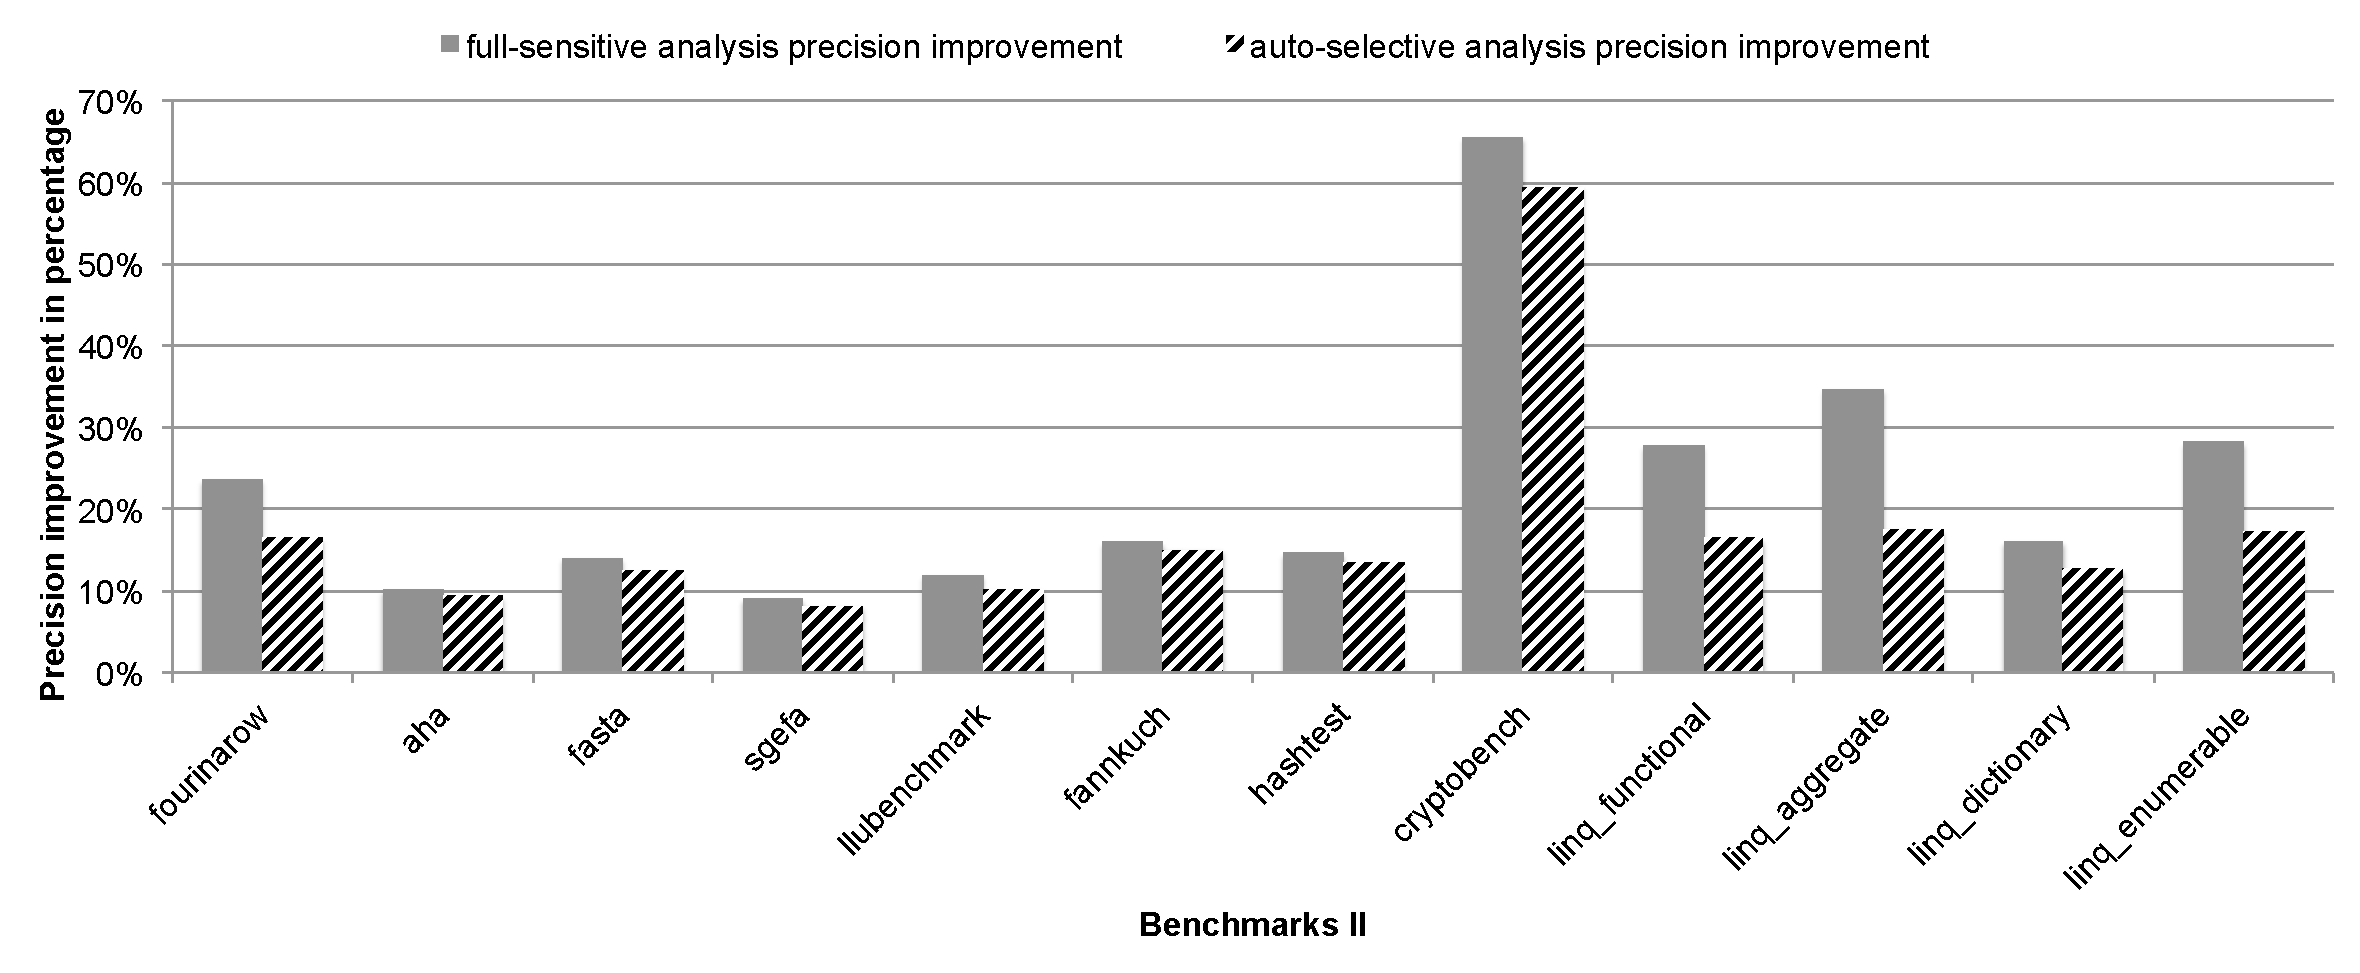
\includegraphics[width=2\columnwidth]{b2-precision}
\caption{\textmd{Benchmarks II precision results.}}
\vspace{-6pt}
\label{fig:b2-precision}
%\vspace{-6pt}
\end{figure*}

\subsection{Benchmarks II Results}
\label{b2-res}

Figures \ref{fig:b2-precision} and \ref{fig:b2-performance} show the precision and performance results of Benchmarks II, respectively. Because the 0-1-CFA analysis finishes analyzing all 12 programs in Benchmarks II within the time budget of 10 minutes, the root-cause localization was performed after the 0-1-CFA points-to analysis completes on each program.

Figure \ref{fig:b2-precision} presents the {\tt PTS\_SIZE} precision improvement of the {\it full-sensitive} analysis (i.e., grey bars) and the {\it auto-selective} analysis (i.e., patterned bars) over the 0-1-CFA analysis. Because the {\it full-sensitive} analysis applies 1-CFA and argument sensitivity of all arguments over all the functions, its results are at least as precise as the {\it selective} analysis. In Figure \ref{fig:b2-precision}, the y axis shows the precision improvement of the corresponding analysis {\tt Y} over the 0-1-CFA analysis {\tt 0-1-CFA}, calculated as follows

\[
  {\tt IMP_{Y} = {{PTS\_SIZE_{0-1-CFA} - PTS\_SIZE_{Y}} \over {PTS\_SIZE_{0-1-CFA}}} \times 100\%}
\]

Therefore, {\tt IMP\textsubscript{Y}} measures analysis {\tt Y}'s precision in terms of removing the false positives from the 0-1-CFA analysis results. In Figure \ref{fig:b2-precision}, the {\it whole-combined} analysis improves the {\tt PTS\_SIZE} precision over the 0-1-CFA analysis by between 9\% (for {\it sgefa}) to 65\% (for {\it cryptobench}). For all but five programs (i.e., {\it fourinarow}, {\it cryptobench}, {\it linq\_functional}, {\it linq\_aggregate} and {\it linq\_enumerable}), the differences of the precision improvement percentages are within 3.5\% between the {\it full-sensitive} and the {\it auto-selective} analyses, indicating that the {\it auto-selective} analysis produces similar results to the {\it full-sensitive} analysis for most programs. The results of the {\it linq\_functional} program exhibit the largest difference in terms of precision improvement (i.e., 17\%) between the {\it full-sensitive} 35\%) and the {\it auto-selective} (18\%) analyses. Nevertheless, more than 50\% of the false positives that are produced by the 0-1-CFA analysis, but not the {\it full-sensitive} analysis, are absent from the {\it auto-selective} analysis results for this program.

Figure \ref{fig:b2-performance} presents the performance results of the {\it full-sensitive} (i.e., grey bars) and the {\it auto-selective} (i.e., patterned bars) analyses comparing to the 0-1-CFA analysis performance. The y axis shows the overhead of the corresponding analysis {\tt Y}'s time cost comparing to the 0-1-CFA analysis time (i.e., ${\tt \frac{TIME_{Y}}{TIME_{0-1-CFA}}}$). The performance of an analysis on each benchmark program was obtained by averaging over 30 repeated executions.

\begin{figure*}[th!]
        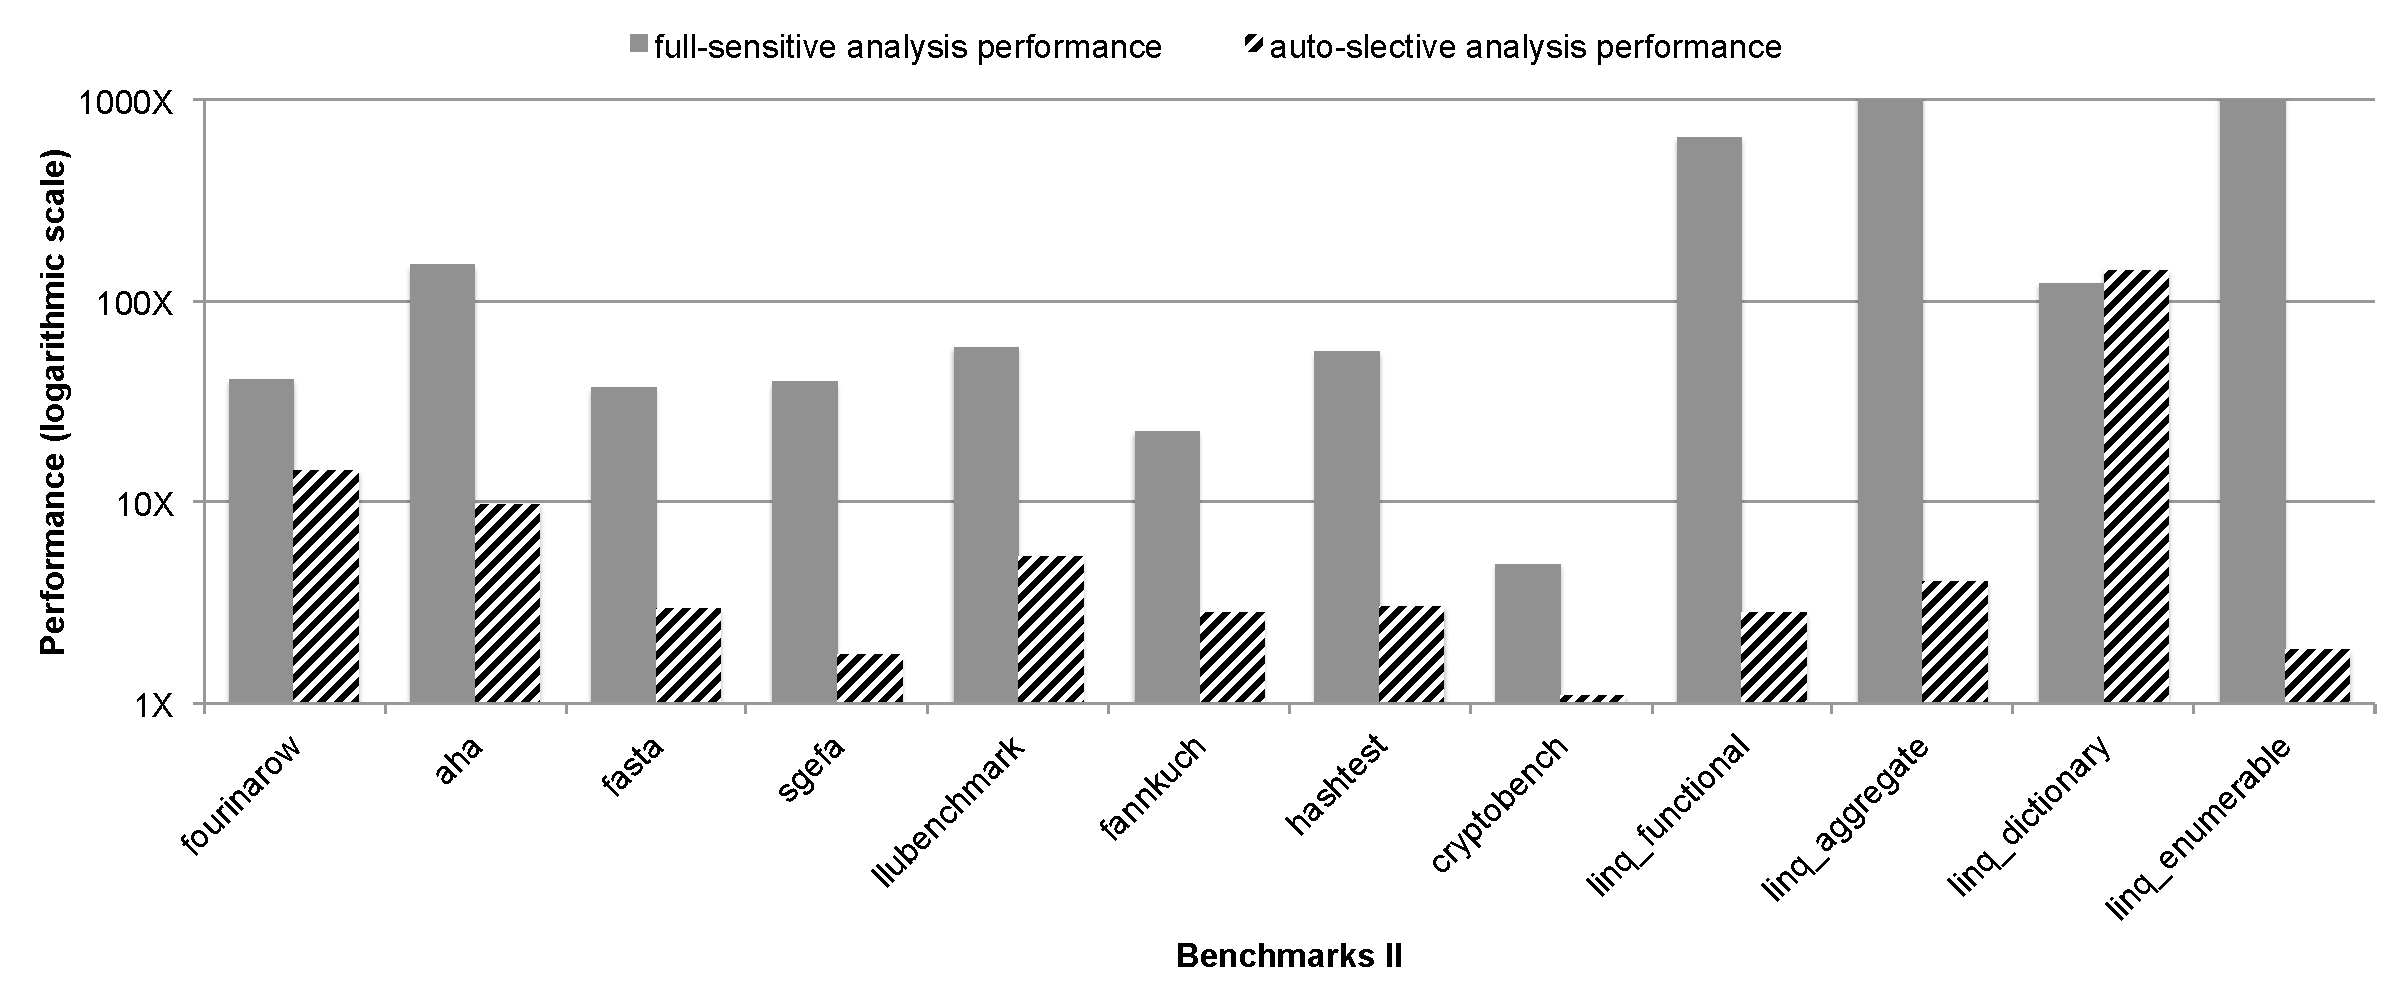
\includegraphics[width=2\columnwidth]{b2-performance}
\caption{\textmd{Benchmarks II performance results.}}
\vspace{-6pt}
\label{fig:b2-performance}
%\vspace{-6pt}
\end{figure*}

In Figure \ref{fig:b2-performance}, the {\it full-sensitive} analysis performs significantly worse than the 0-1-CFA analysis for all the benchmark programs. It could not finish analyzing {\it linq\_aggregate} and {\it linq\_enumerable} under the time budget of 10 minutes; therefore, the incomplete points-to results of these two programs were obtained after the timeout for comparison. The {\it full-sensitive} analysis is at least two orders of magnitude slower for another three program (i.e.,  {\it linq\_functional}, {\it aha}, and {\it linq\_dictionary}) and is between 23 (for {\it fannkuch}) and 60 (for {\it llubenchmark}) times slower for six programs than the 0-1-CFA analysis. For example, it takes less than one second for the 0-1-CFA analysis to finish analyzing {\it linq\_functional}, while the {\it full-sensitive} analysis needs almost 7 minutes to complete analyzing the same program. Despite of the fact that the {\it full-sensitive} analysis often results in relatively significant precision improvement (e.g., 28\% for {\it linq\_functional}), the performance issues outweigh the benefits of this whole-program combined context-sensitive analysis in many cases.

%, for 4 programs (i.e., {\it fourinarow}, {\it aha}, {\it sgefa} and {\it llubenchmark}) about 100 times slower and another 5 programs ({\it frannkuch}, {\it hashtest}, {\it linq\_aggregate}, {\it linq\_dictionary} and {\it linq\_enumerable}) about an order of magnitude slower. For example, it takes less than one second for the 0-1-CFA analysis to finish analyzing {\it fourinarow}, while the {\it whole-combined} analysis needs about 2 minutes to complete analyzing the same program. Despite of the fact that the {\it whole-combined} analysis often results in relatively significant precision improvement (e.g., 19.6\% for {\it fourinarow}), the performance issues outweigh the benefits of this whole-program combined context-sensitive analysis in many cases.

On the other hand, the {\it auto-selective} analysis is capable of analyzing the benchmarks under the same order of magnitude as the 0-1-CFA analysis for all but three programs (i.e., {\it fourinarow}, {\it aha} and {\it linq\_dictionary}). For example, the {\it auto-selective} analysis improves the precision over the 0-1-CFA analysis by 59\% for {\it cryptobench} and it also finishes analyzing this program almost as fast as the 0-1-CFA analysis. In most cases, the {\it auto-selective} analysis results in a much better balance between performance and precision than the {\it full-sensitive} analysis (e.g., the {\it full-sensitive} analysis is 65\% more precise but performs 5 times slower than the 0-1-CFA analysis for {\it cryptobench}). For three programs the {\it auto-selective} analysis performs more than 10 times slower than the 0-1-CFA analysis (i.e., 10, 15 and 143 times slower for {\it aha}, {\it fourinarow} and {\it linq\_dictionary}, respectively), the {\it auto-selective} analysis is still an order of magnitude faster than the {\it full-sensitive} analysis for {\it aha} and about 3 times faster than the {\it full-sensitive} analysis for {\it fourinarow}. An outlier is the performance of the {\it auto-selective} analysis for {\it linq\_dictionary}, which is similar to the {\it full-sensitive} analysis in performance for {\it linq\_dictionary}, indicating the {\it auto-selective} analysis may have applied expensive context sensitivity on a set of functions that result in performance overhead. Nevertheless, the {\it auto-selective} analysis has achieved significantly better performance than the {\it full-sensitive} analysis for most of the programs in Benchmarks II.

Our localization algorithm identifies between 6\% (for {\it fourinarow}) to 27\% (for {\it linq\_aggregate}) of the functions as the sources of precision loss, with an average of 13\% of the functions over all the programs in Benchmarks II, a relatively small fraction. Our improvement suggestion algorithm recommends 72\%, 25\%, and 3\% of all the root cause functions in Benchmarks II to apply a combined context-sensitive analysis, a single context-sensitive analysis and a context-insensitive analysis, respectively.

In summary, the {\it auto-selective} analysis obtains similar precision results to the {\it full-sensitive} analysis that improves the precision of the 0-1-CFA analysis; moreover, the {\it auto-selective} analysis' performance is significantly better than the whole-program combined fully context-sensitive analysis. This result suggests that our localization algorithm can accurately identify the small fraction of functions as root causes and our improvement suggestion algorithm can suggest the appropriate context sensitivity that benefit the results both in performance and precision for Benchmarks II.

%\subsection{Case Study}
%\label{case-study}

%\subsection{Discussion}

\section{Related Work}
\label{related}


\section{Conclusions}

\bibliographystyle{abbrv}
\bibliography{main}

\end{document}
